\chapter{Codifica di sorgente}

Tratteremo ora il caso di un canale completamente affidabile (come quello in figura \ref{fig:0006}). Non essendoci alcun disturbo, ogni 
simbolo inviato corrisponderà a quello ricevuto. Siamo interessati a ``compattare'' l'informazione il più possibile, eliminando
la ridondanza. Come già enunciato nell'introduzione, l'eliminazione della ridondanza consente di comprimere l'informazione. In questo modo potremo aumentare la velocità di trasmissione (ci sono infatti meno simboli da mandare).

\begin{definizione}[codice di sorgente] 
Sia X una variabile aleatoria, con \(\X = \{x_1 ... x_k\}\), caratterizzata da una certa distribuzione di probabilità nota:
\[X \sim p(x) \ \forall x \in X\]
e sia $\D$ un alfabeto D-ario finito, $\D=\{0,1,..,D-1\}$. Allora si dice codice di sorgente una funzione che assegna a ciascun simbolo della variabile casuale X una stringa di simboli appartenenti all'alfabeto D:
\[C: \X \longrightarrow \D^*\]
\end{definizione}
Dove \(\D*\) indica l'insieme di tutte le sequenze di qualsiasi lunghezza costruita su simboli di D, ossia:
\[\D^* = \cup_{k = 1}^\infty \D^k\]
con \(\D^k\) insieme delle stringhe di lunghezza k:
\[\D^k = \begin{matrix}  \underbrace{\D \times \D ... \times \D} \\ k
\end{matrix}\]

In tabella \ref{tab:codici1} sono riportati alcuni esempi di codici. In questo caso è stato utilizzato un alfabero 
binario, ovvero $\D=\{0,1\}$. Mentre $X=\{a,b,c,d\}$. Gli elementi del codominio della funzione del codice, sono detti ``parole di codice'' (codewords). Nell'esempio di $C^I$, le parole di codice sono 0,00,10,1101.


\begin{table}[htbp]
  \begin{center}
   \begin{tabular}{c|c}
	$C^I$ & $C^{II}$ \\
       \hline
	$a \to 0$ & $a \to 0$ \\ 
	$b \to 00$ & $b \to 00$ \\ 
	$c \to 10$ & $c \to 10$ \\ 
        $d \to 1101$ & $d \to 1101$ \\ 
    \end{tabular}
     
     \caption{Esempio di codici}
    \label{tab:codici1}
  \end{center}
\end{table}

E' naturale chiedersi quando un codice sia preferibile rispetto ad un altro.
Possiamo esprimere la bontà di un codice in base a due parametri: la sua lunghezza media (che deve essere più piccola possibile) e l'efficacia con cui il destinatario può ricostruire il messaggio ricevuto; un codice deve quindi avere due caratteristiche:
\begin{enumerate}
\item non ambiguità
\item efficienza
\end{enumerate}

Per chiarire meglio questa idee, consideriamo i codici in tabella \ref{tab:codici2}: 
\begin{itemize}
 \item Il codice 3 è molto efficiente (utilizza per ogni lettera un solo simbolo). Tuttavia è molto ambiguo, quanto infatti
 il destinatario riceve 0 non è in grado di determinare se sia stata inviata una a o una b.
 \item Il codice 4 è poco efficiente (sequenze molto lunghe), tuttavia non è ambiguo. Il destinatario sarà infatti in grado di 
determinare il simbolo inviato dalla sorgente.
 \item Il codice 5 rispetta invece entrambi i criteri. Non si utilizzano molti simboli e non si ha ambiguità.
\end{itemize}

\begin{table}[htbp]
  \begin{center}
   \begin{tabular}{c|c|c}
	$C^{III}$ & $C^{IV}$ & $C^{V}$\\
       \hline
	$a \to 0$ & $a \to 1101$ & $a \to 0$ \\ 
	$b \to 0$ & $b \to 110000$ & $b \to 10$ \\ 
	$c \to 1$ & $c \to 00100$ & $c \to 110$ \\ 
        $d \to 1$ & $d \to 11111$ & $d \to 111$ \\ 
    \end{tabular}
     
     \caption{Esempio di codici}
    \label{tab:codici2}
  \end{center}
\end{table}

Quantifichiamo ora con più precisione il concetto di efficienza di un codice.
In particolare misureremo questa efficienza, calcolando la lunghezza media delle parole del codice.

\begin{definizione}[lunghezza di un codice sorgente] 
\mbox{}

Dato un codice di sorgente C:
\[C: \X \longrightarrow \D*\]
La sua lunghezza (media) è:
\[L(C) = \sum_{x \in \X}l(x) p(x)\]
Dove con l(x) abbiamo indicato la lunghezza della parola di codice x.
\label{lunghezza}
\end{definizione}

\noindent
\textbf{Esempio}

\noindent
Prendiamo in considerazione il codice $C^V$ (tabella \ref{tab:codici2}) e calcoliamo la sua lunghezza.
Per poterlo fare, assumiamo che la variabile X sia distribuita nel modo seguente:

\[X = \left(\begin{array}{cccc}a & b & c & d \\1/2 & 1/4 & 1/8 & 1/8\end{array}\right)\]

Risulta dunque:
\[L(C) = 1/2 \cdot 1 + 1/4 \cdot 2 + 1/8 \cdot 3 + 1/8 \cdot 3 = 7/4 = 1,75\]

E' ora interessante provare a calcolare l'entropia della variabile X:
\[
\begin{split}
H(X)&= \sum_{x \in \X}l(x) \log \frac{1}{p(x)} = \\
&= 1/2 \cdot \log 2^1 + 1/4 \cdot \log 2^2 + 1/8 \cdot \log 2^3 + 1/8 \cdot \log 2^3 = \\
&= 1/2 \cdot 1 + 1/4 \cdot 2 + 1/8 \cdot 3 + 1/8 \cdot 3 = \\
&= 7/4 = 1,75
\end{split}
\]

Come si può vedere, succede che l'entropia coincide con la lunghezza del codice. Si tratta di un caso particolare (dovuto
alla scelta del codice). Come vedremo successivamente, l'entropia rappresenta un limite inferiore alla lunghezza di un codice.

\section{Tipi di codice}
Abbiamo definito come misurare quantitativamente l'efficienza di un codice (in base alla sua lunghezza media).
Vediamo ora come formalizzare l'ambiguità.

\begin{definizione}[codice non singolare] 
Un codice C si dice \textit{non singolare} se C (in quanto funzione) è \textbf{iniettiva}. 
Ossia se presi due simboli \(x_1 \ e \ x_2\):
\[x_1 \neq x_2 \Rightarrow C(x_1) \neq C(x_2)\]
ossia per simboli diversi, si hanno parole di codice diverse.
\end{definizione}

\noindent
\textbf{Esempio}
Il codice \(C^{III}\) in tabella \ref{tab:codici2} è singolare. I codici $C^{IV}$ e $C^{V}$, invece, sono non singolari.

\bigskip
\noindent
Come è facile notare, il fatto di avere un codice non singolare, non garantisce l'assenza di ambiguità. Si consideri ad esempio il codice in figura \ref{fig:codice3}. Il destinatario vede arrivare una sequenza continua di simboli e deve essere in grado di distinguere le varie stringhe. Nell'esempio tuttavia sorgono dei problemi. Se si riceve '010' non si è in grado di stabilire se è stato inviato b oppure c seguito do a. Un codice non ambiguo, deve essere quindi caratterizzato da una \textbf{segmentazione non ambigua}.

\begin{figure}[htbp]
\begin{center}
	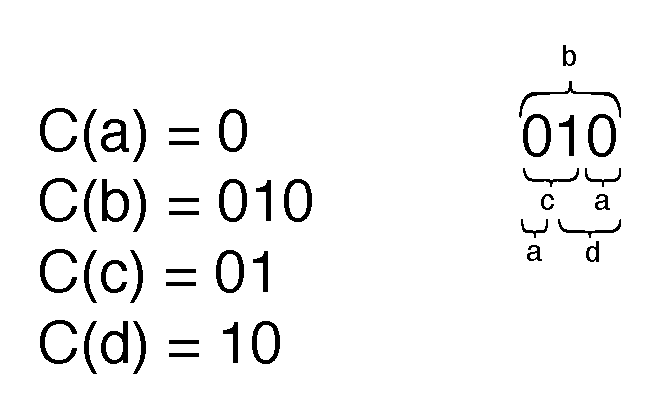
\includegraphics[width=0.4\textwidth]{img/codice3.pdf}
\caption{esempio di codice non singolare ma ambiguo; si può notare a destra come la segmentazione presenti delle ambiguità: la stringa 010 potrebbe infatti essere interpretata come b oppure come c seguito da a, oppure come a seguita da d.}
\label{fig:codice3}
\end{center}
\end{figure}

Abbiamo in sostanza bisogno di un criterio più forte per costruire codici non ambigui.
Se C è un codice qualsiasi, la sua estensione k-esima è un codice costruito su stringhe di simboli di X lunghe k:
\[C^k: \X^k \longrightarrow \D^*\]
dove:
\[C^k(x_1... x_k) = C(x_1) C(x_2) ... C(x_k)\]
Consideriamo il codice in figura \ref{fig:codice3}. La sua estensione 2\textordfeminine \ sarà quella rappresentata in tabella \ref{tab:codice4}.

\begin{table}[htbp]
  \begin{center}
   \begin{tabular}{c|c}
	$\X^{2}$ & $ \D^{*}$ \\
       \hline
	$aa$ & $00$ \\ 
	$ab$ & $0010$ \\ 
	$ac$ & $001$ \\ 
        $ad$ & $010$ \\ 
        $ba$ & $0100$ \\ 
        $...$ & $...$ \\ 
    \end{tabular}
     
     \caption{Estensione 2° del codice}
    \label{tab:codice4}
  \end{center}
\end{table}

A partire dall'estensione k-esima possiamo quindi costruire l'estensione, ossia quella che mappa una qualsiasi stringa costruita su simboli di \(\X\) in $D^*$:
\[C^*: \X^* -> \D^*\]
\[C^*(x_1... x_n) = C(x_1) C(x_2) ... C(x_n)\]

\begin{definizione}[Codice U.D.]
Sia \(C: \X \longrightarrow \D^*\) un codice, C si dice \textit{univocamente decodificabile} (UD) se:
\[C^*: \X^* \longrightarrow \D^*\]
(l'\textit{estensione del codice}), è non singolare.
\label{codiceUD}
\end{definizione}

Se un codice è UD, allora il destinatario riuscirà sempre a segmentare i bit in arrivo.
Riprendendo sempre l'esempio precedente, appare chiaro che il codice in figura \ref{fig:codice3} non è UD Infatti nella sua estensione 2° (tabella \ref{tab:codice4}) compare la sequenza '010', che però è presente anche nel codice originale (figura \ref{fig:codice3}).


I codici UD sono sicuramente non ambigui, ma alcuni di essi possono essere inefficienti, come quello rappresentato in figura \ref{fig:0024}: in questo caso il fatto che una parola sia prefisso dell'altra provoca l'introduzione di un ritardo di decodifica. Ciò è dovuto al fatto che è necessario un certo numero di simboli per riuscire a distinguere le due differenti parole. Per ovviare a questo problema introduciamo un'ulteriore classe di codici.

\begin{figure}[htbp]
\begin{center}
	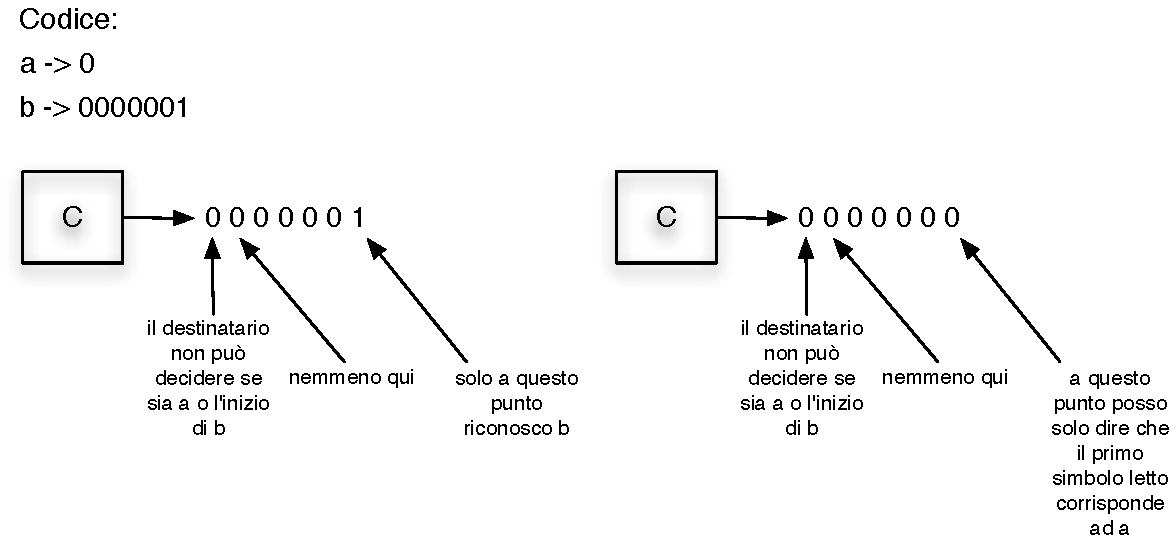
\includegraphics[width=\textwidth]{img/istantaneo.pdf}
\caption{esempio di codice UD poco efficiente (si tratta di un comma code, in quanto l'1 funge da separatore delle stringhe)}
\label{fig:0024}
\end{center}
\end{figure}

\begin{figure}[htbp]
\begin{center}
	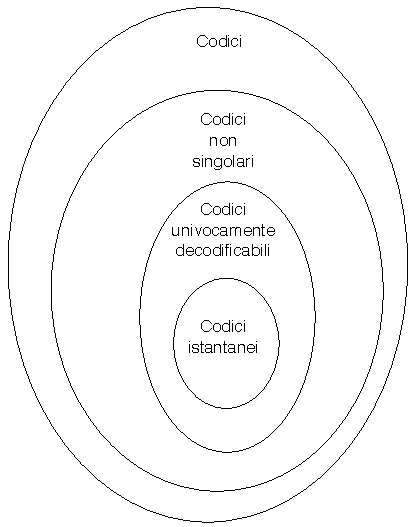
\includegraphics[width=0.5\textwidth]{img/codici.pdf}
\caption{schema riassuntivo dei tipi di codice}
\label{fig:0004}
\end{center}
\end{figure}


\begin{definizione}[codice istantaneo]
Un codice C si dice \textit{istantaneo o a prefisso} se nessuna parola di codice è prefisso di un'altra.
\end{definizione}
Possiamo osservare che un codice istantaneo è sicuramente anche UD (torneremo meglio dopo su questo punto). In sostanza i codici 
istantanei sono un sottoinsieme di quelli UD. Possiamo anche dire che è necessario avere un codice UD (per non avere ambiguità), tuttavia è preferibile che il codice sia anche istantaneo (più efficienza).
In figura \ref{fig:0004} è rappresentato uno schema riassuntivo dei codici visti.





\subsection{Teorema di Sardinas-Patterson}
Non è sempre immediato determinare se un codice sia o meno univocamente decodificabile, in quanto bisognerebbe considerare la sua estensione (che come abbiamo visto è formata da stringhe di lunghezza infinita).
E' necessario quindi un criterio che renda questa operazione più semplice. Il teorema di Sardinas-Patterson fornisce un metodo utile.

L'idea base del teorema è la seguente. Supponiamo di avere una stringa binaria di un codice non UD (figura \ref{fig:0018}): ciascuna parola della segmentazione in alto ha il suffisso che è anche prefisso delle corrispondenti parole nella segmentazione in basso; il problema si verifica quando il suffisso di una parola della segmentazione in alto coincide con una parola intera della segmentazione alternativa, perchè questo può dar luogo a una doppia interpretazione. Se invece le segmentazioni si intersecano sempre, senza mai che un suffisso e una parola coincidano, allora il codice è UD.

\begin{figure}[htbp]
\begin{center}
	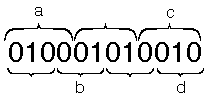
\includegraphics[width=0.4\textwidth]{img/ud.pdf}
\caption{a ha il suffisso che è prefisso di b; c ha il suffisso che coincide con l'intera parola d}
\label{fig:0018}
\end{center}
\end{figure}

\begin{teorema}[di Sardinas-Patterson]
Dato un codice \(C: X -> \D^*\), e posti:
\[S_0 = C(X_0) = \{C(x) \in \D^* | x \in X_0\}\]
\[\forall \ n \geq 1 : S_n = \{w \in D^* | \exists \ a \in S_0, \exists \ b \in S_{n-1} \ t.c. \  a = bw \lor b = aw\}\]
(ossia l'insieme dei suffissi), allora condizione necessaria e sufficiente affinchè C sia univocamente decodificabile è:
\[\forall \ n \geq 1 : S_0 \cap S_n = \varnothing\]
ossia nessuno dei suffissi generati dovrà corrispondere con una parola di codice.
\end{teorema}

Perchè un codice sia UD bisogna verificare la condizione per qualsiasi valore di n, quindi dovremmo iterare il procedimento fino a trovare il primo n per cui la condizione è violata. Ma questo potrebbe non accadere mai (e questo è ovvio nel caso in cui si stia analizzando un codice UD), e quindi l'algoritmo itererebbe all'infinito. Tuttavia l'insieme dei suffissi generabili è finito, quindi il processo prima o poi comincerà a generare insiemi già generati: in tal caso la procedura termina (e il codice è UD). Può verificarsi anche il caso in cui a un certo punto si genera l'insieme vuoto: anche qui la procedura termina e il codice è UD (da ora in poi saranno tutti insiemi vuoti).

\bigskip
\noindent
\textbf{Esempio}

\noindent
Verifichiamo se il codice ($S_0$ in figura \ref{fig:0019}) è UD: il procedimento è rappresentato sempre in figura \ref{fig:0019}:
\begin{enumerate}
\item \(S_0\) è il codice di partenza;
\item per costruire \(S_1\) vado a vedere se qualche parola di \(S_0\) è prefisso di qualcun'altra nello stesso insieme; se ne trovo vado a prendere il suffisso e lo metto in \(S_1\): a è prefisso di ab e abb, quindi inseriamo in \(S_1\) i corrispondenti suffissi d e bb;
\item controllo se gli elementi di \(S_1\) ci sia una parola di codice, cosa non vera, per cui proseguo;
\item per costruire \(S_2\) vado a vedere se qualche parola di \(S_1\) è prefisso di qualche parola di \(S_0\) o se qualche parola di \(S_0\) è prefisso di qualche parola di \(S_1\); se ne trovo vado a prendere il suffisso e lo metto in \(S_1\): d è prefisso di deb, mentre bb di bbcde, quindi inseriamo in \(S_2\) i corrispondenti suffissi eb e cde;
\item controllo se gli elementi di \(S_2\) ci sia una parola di codice, cosa non vera, per cui proseguo;
\item e così via...
\item arrivato ad  \(S_5\) scopro che ad è una parola di codice, quindi possiamo concludere che il codice non è UD.
\end{enumerate}
Altri due esempi di applicazione del teorema di Sardinas-Patterson sono rappresentati nelle figure \ref{fig:0020} e \ref{fig:0021}.

\begin{figure}[htp]
\begin{center}
	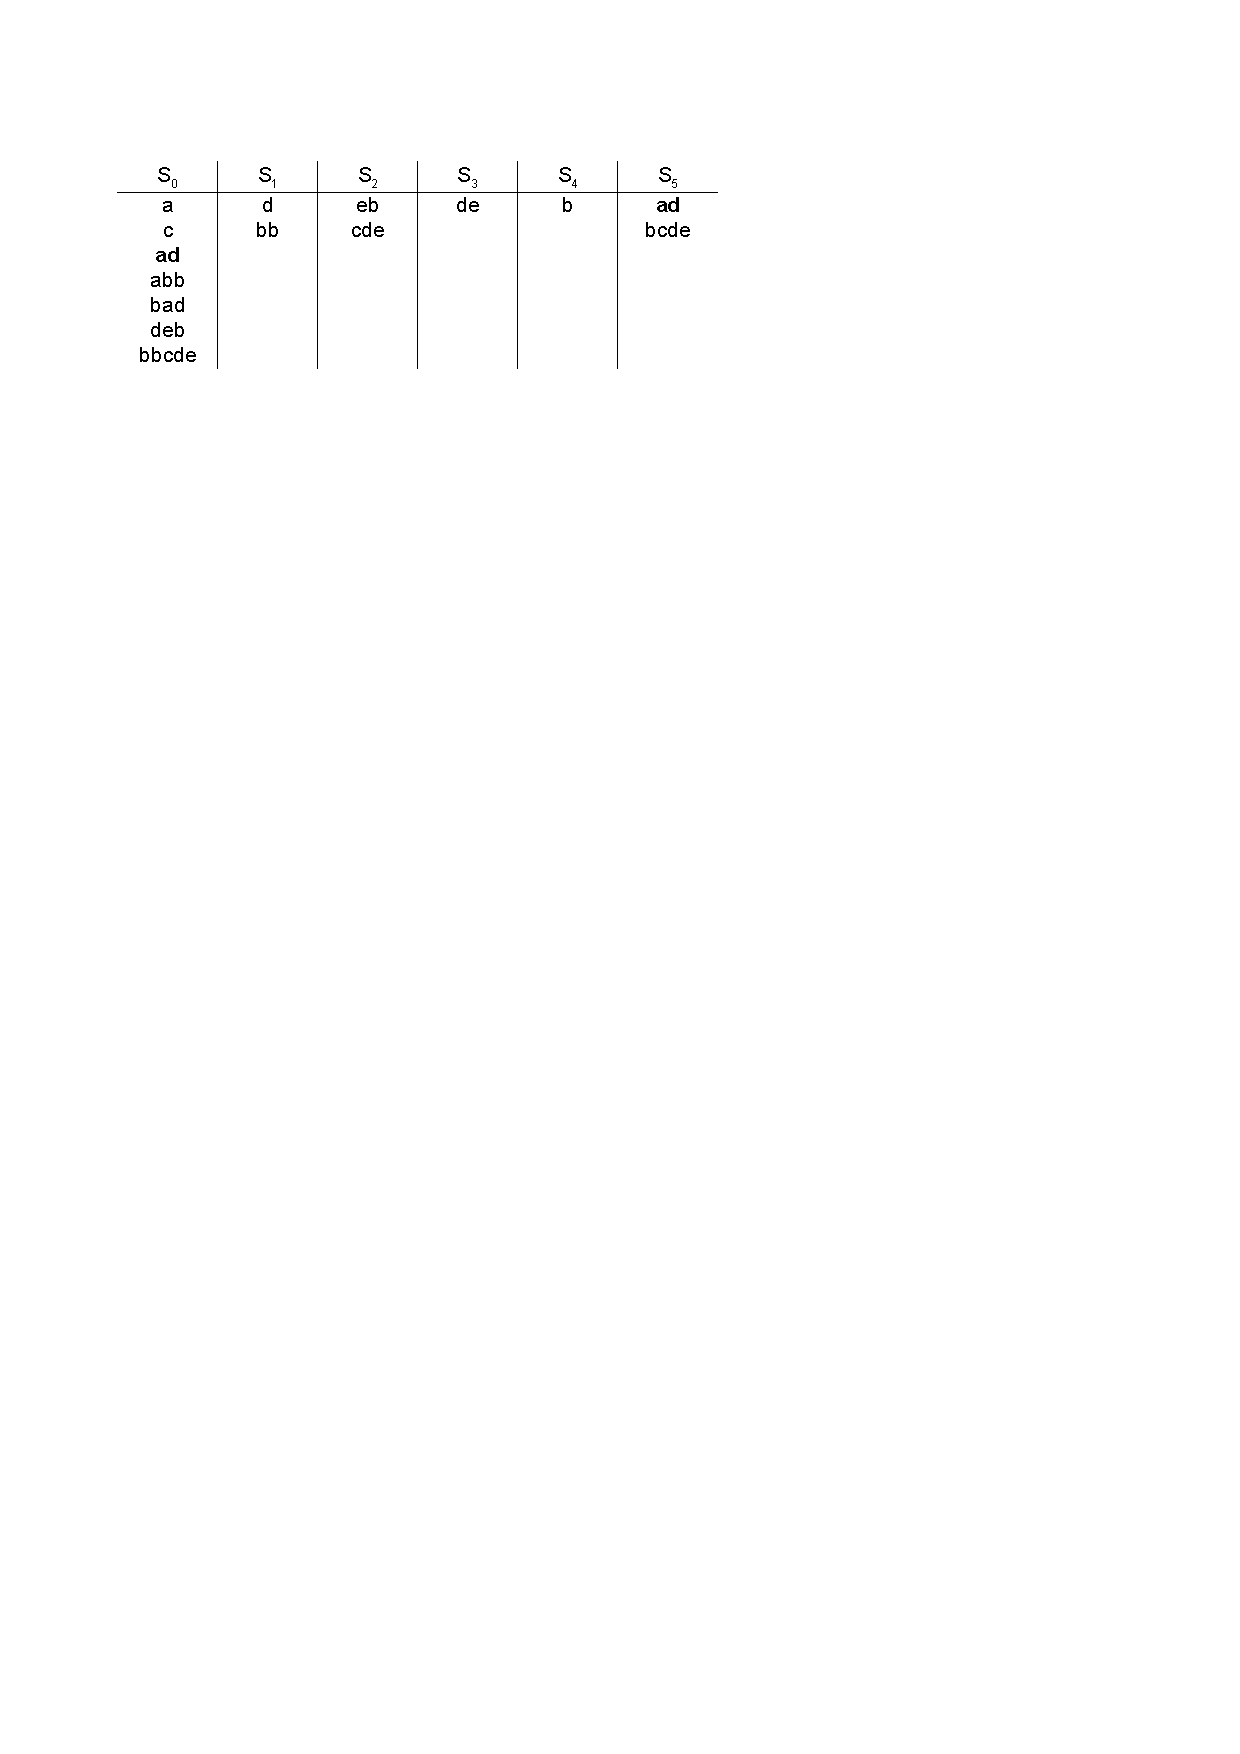
\includegraphics[width=\textwidth]{img/patt1.pdf}
	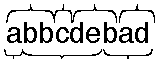
\includegraphics[width=0.2\textwidth]{img/patt1b.pdf}
\caption{procedimento basato sul teorema di Sardinas-Patterson; il codice non è UD. In basso un esempio di ambiguità}
\label{fig:0019}
\end{center}
\end{figure}

\begin{figure}[htp]
\begin{center}
	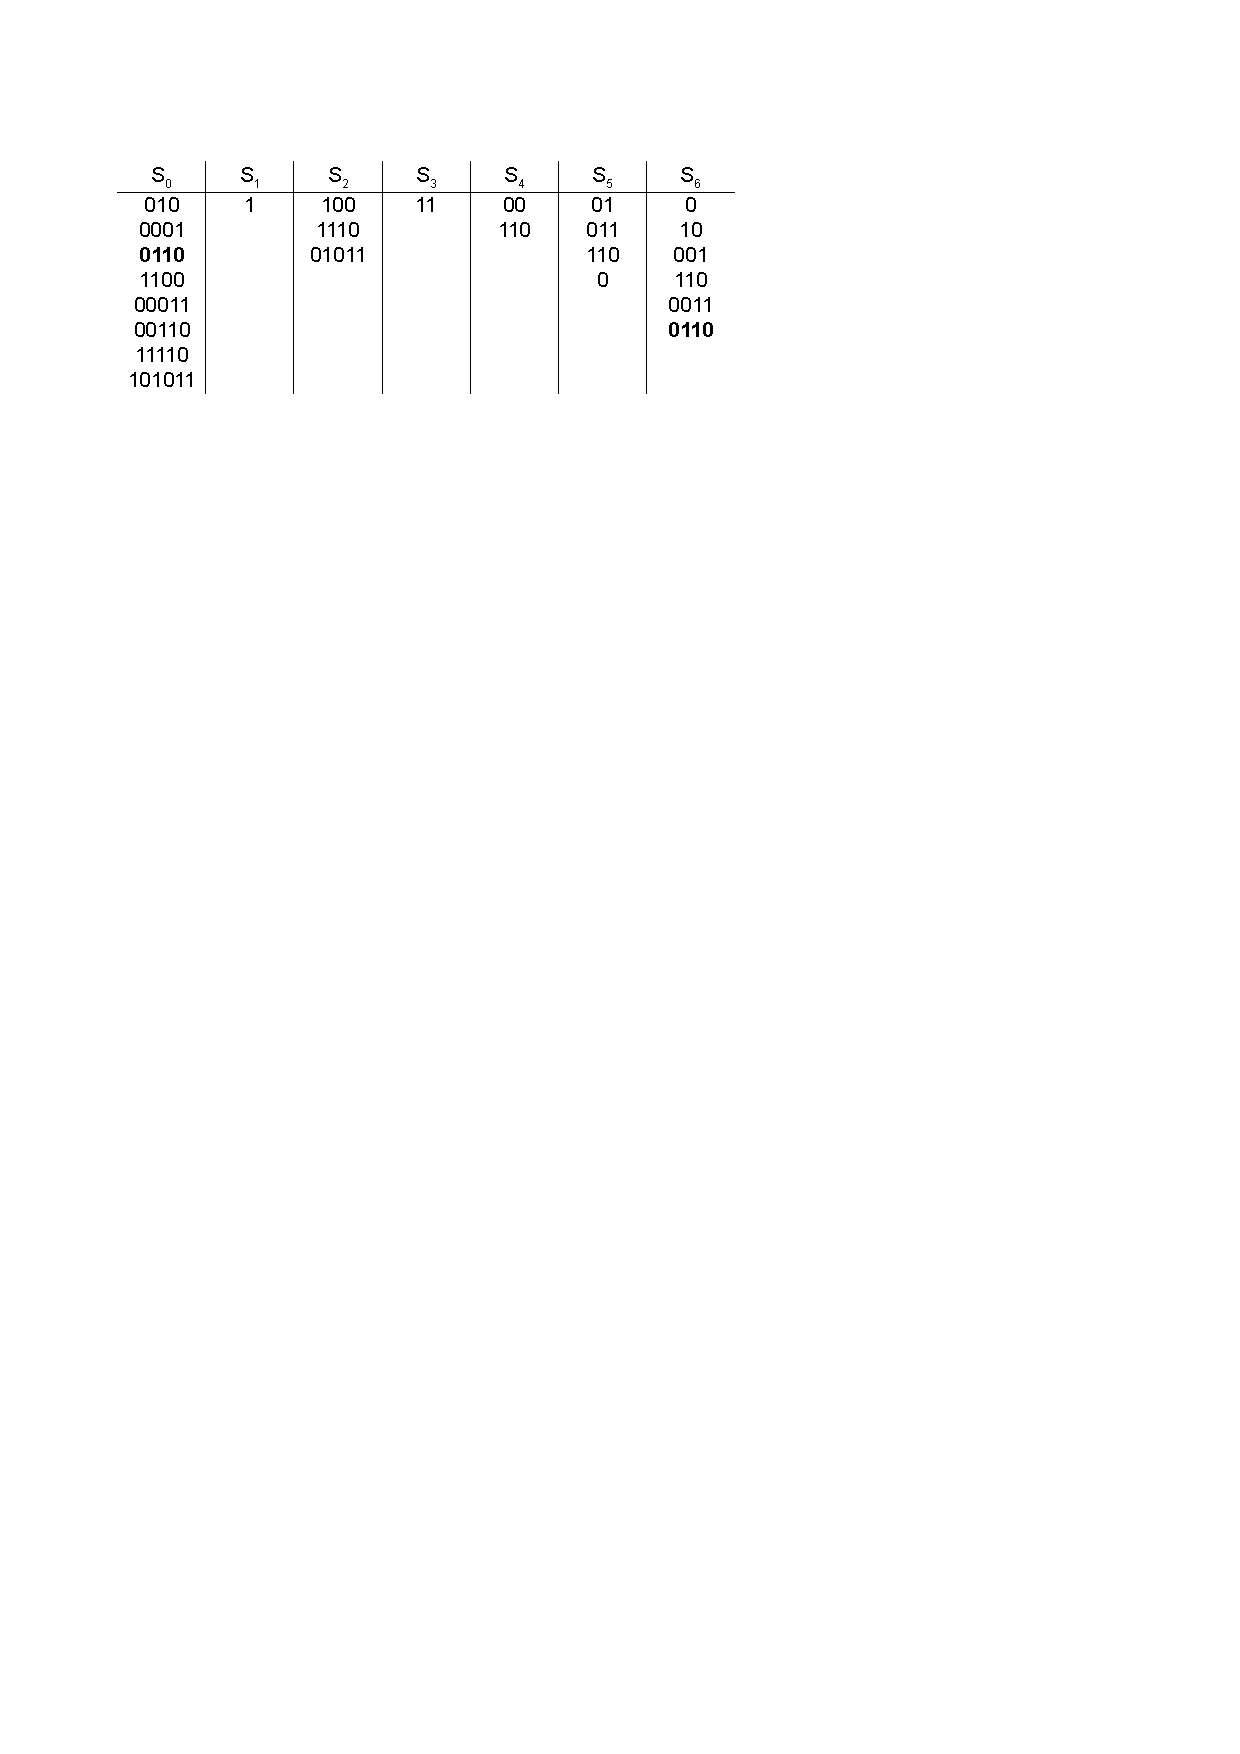
\includegraphics[width=\textwidth]{img/patt2.pdf}
\caption{procedimento basato sul teorema di Sardinas-Patterson, il codice non è UD}
\label{fig:0020}
\end{center}
\end{figure}

\begin{figure}[htp]
\begin{center}
	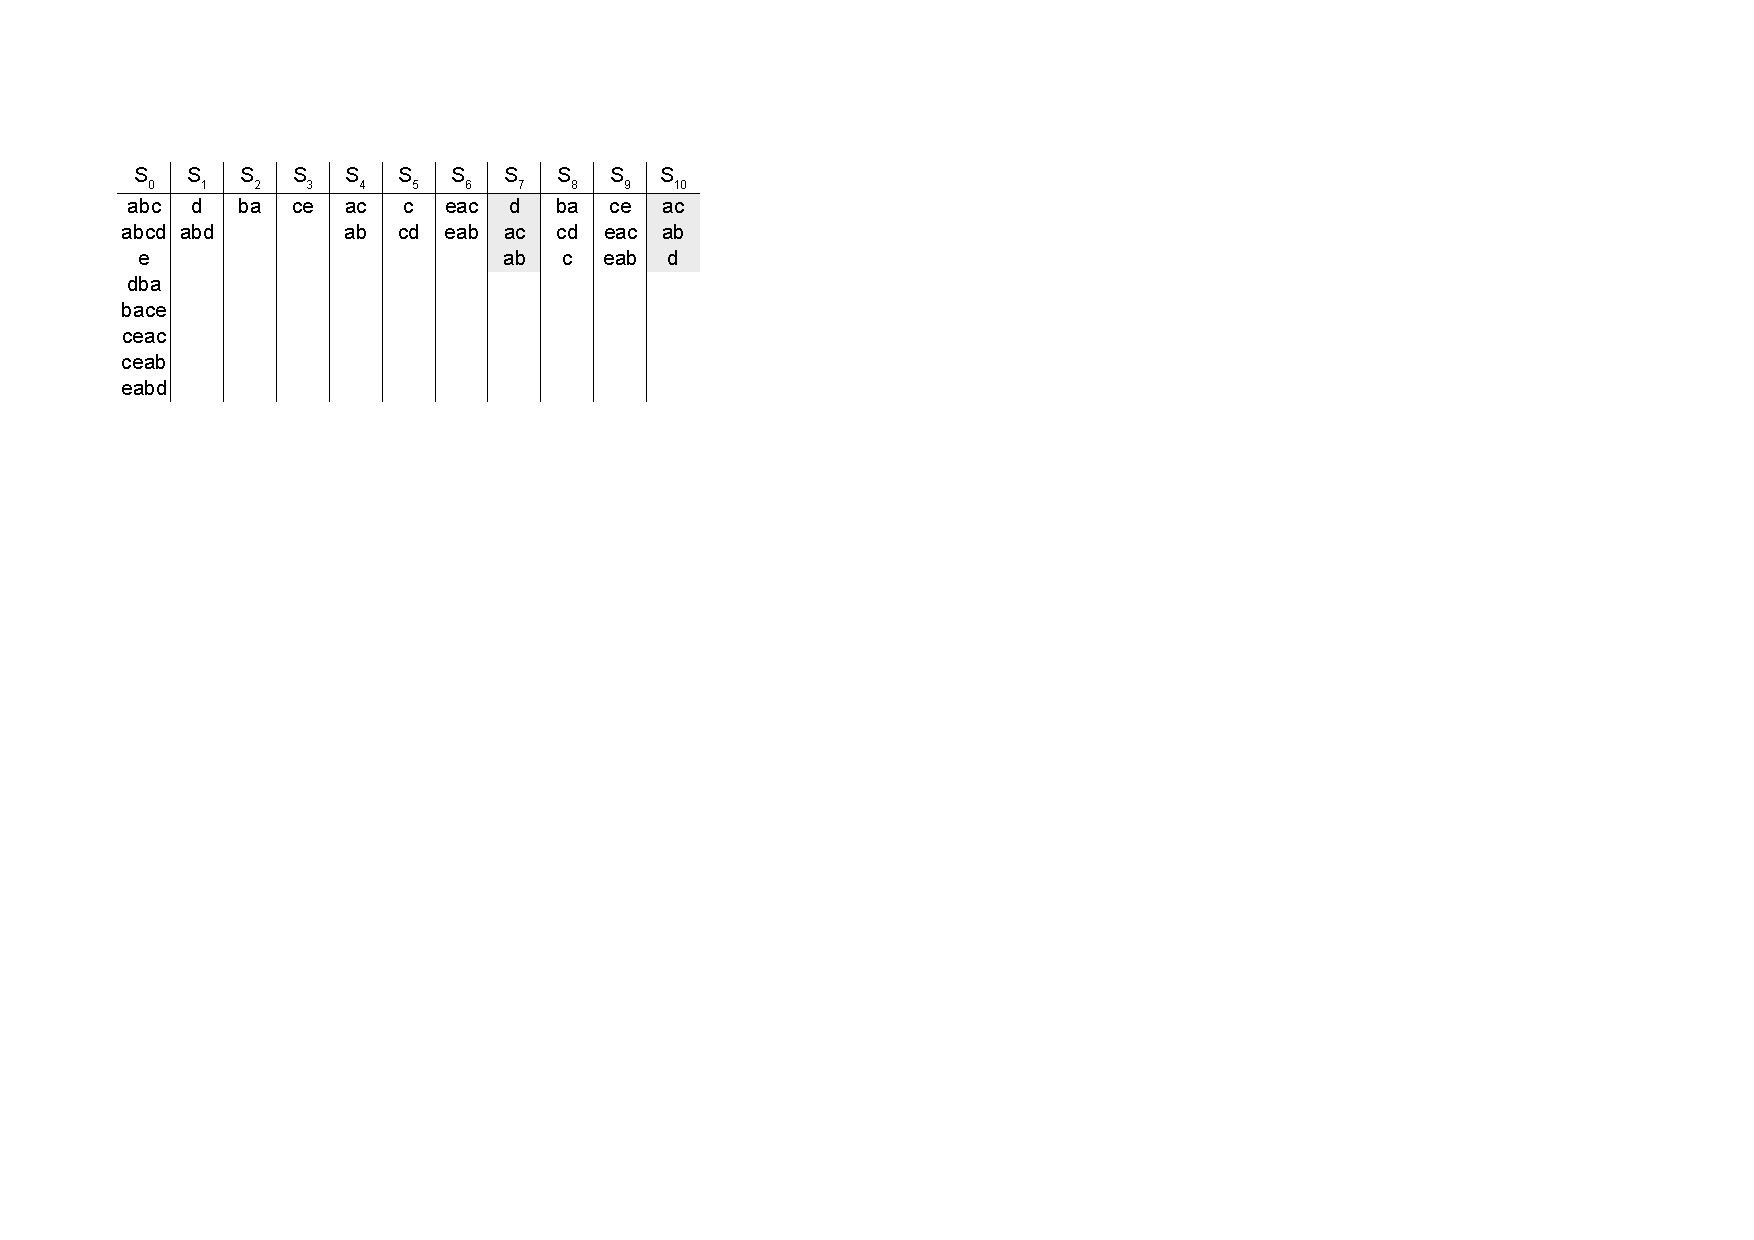
\includegraphics[width=0.9\textwidth]{img/patt3.pdf}
\caption{procedimento basato sul teorema di Sardinas-Patterson, il codice è UD}
\label{fig:0021}
\end{center}
\end{figure}

\newpage

\section{Costruzione di codici}
Sono stati visti vari tipi di codici. Inoltre abbiamo evidenziato come le classi di maggior interesse siano quelle dei codici istantanei 
ed univocamente decodificabili. Vediamo ora quali condizioni devono valere, affinché sia possibile costruirli.

\subsection{Disuguaglianza di Kraft}
La Disuguaglianza di Kraft, fornisce un vincolo importante per la costruzione di codici istantanei.
Infatti, affinché sia possibile costruire un codice istantaneo, la lunghezza delle parole di codice deve rispettare un vincolo.
\`E importante notare che il teorema esprime la possibilità di costruire un codice istantaneo. In altre parole, se il teorema vale allora con determinate lunghezze di parole di codice si può un costruire un codice istantaneo. Tuttavia non tutti i codici con quelle determinate lunghezze sono istantanei!

\begin{teorema}[Disuguaglianza di Kraft]
\label{kraft}
Condizione necessaria e sufficiente \textbf{affinchè sia possibile} costruire un codice istantaneo D-ario (ossia un codice costruito su un alfabeto di D simboli) con lunghezza di parola \(l_1, l_2 ... l_n\) è:
\[\sum_{i = 1}^n D^{-l_i} \leq 1\]
\begin{proof}
A partire da un codice D-ario, possiamo costruire il corrispondente \textbf{albero D-ario di codifica} (figura \ref{fig:albero}).
L'albero ha profondità pari alla lunghezza della parola più grande e ciascun vertice (o ciascun cammino) rappresenterà una sequenza 
di simboli (la cui lunghezza è al massimo la lunghezza della parola più lunga).
Nell'albero si evidenziano i vertici, i cui cammini dalla radice corrispondono ad una parola di codice.
In questo modo si costruisce una corrispondenza biunivoca tra il codice e l'albero.
E' facile osservare che un codice è istantaneo se e solo se nel corrispondente albero di codifica non esistono due vertici evidenziati che appartengono uno al sottoalbero dell'altro. In altre parole, percorrendo il cammino dalla radice ad un vertice evidenziato, non devo incontrare altri vertici evidenziati.

\begin{figure}[htbp]
\begin{center}
	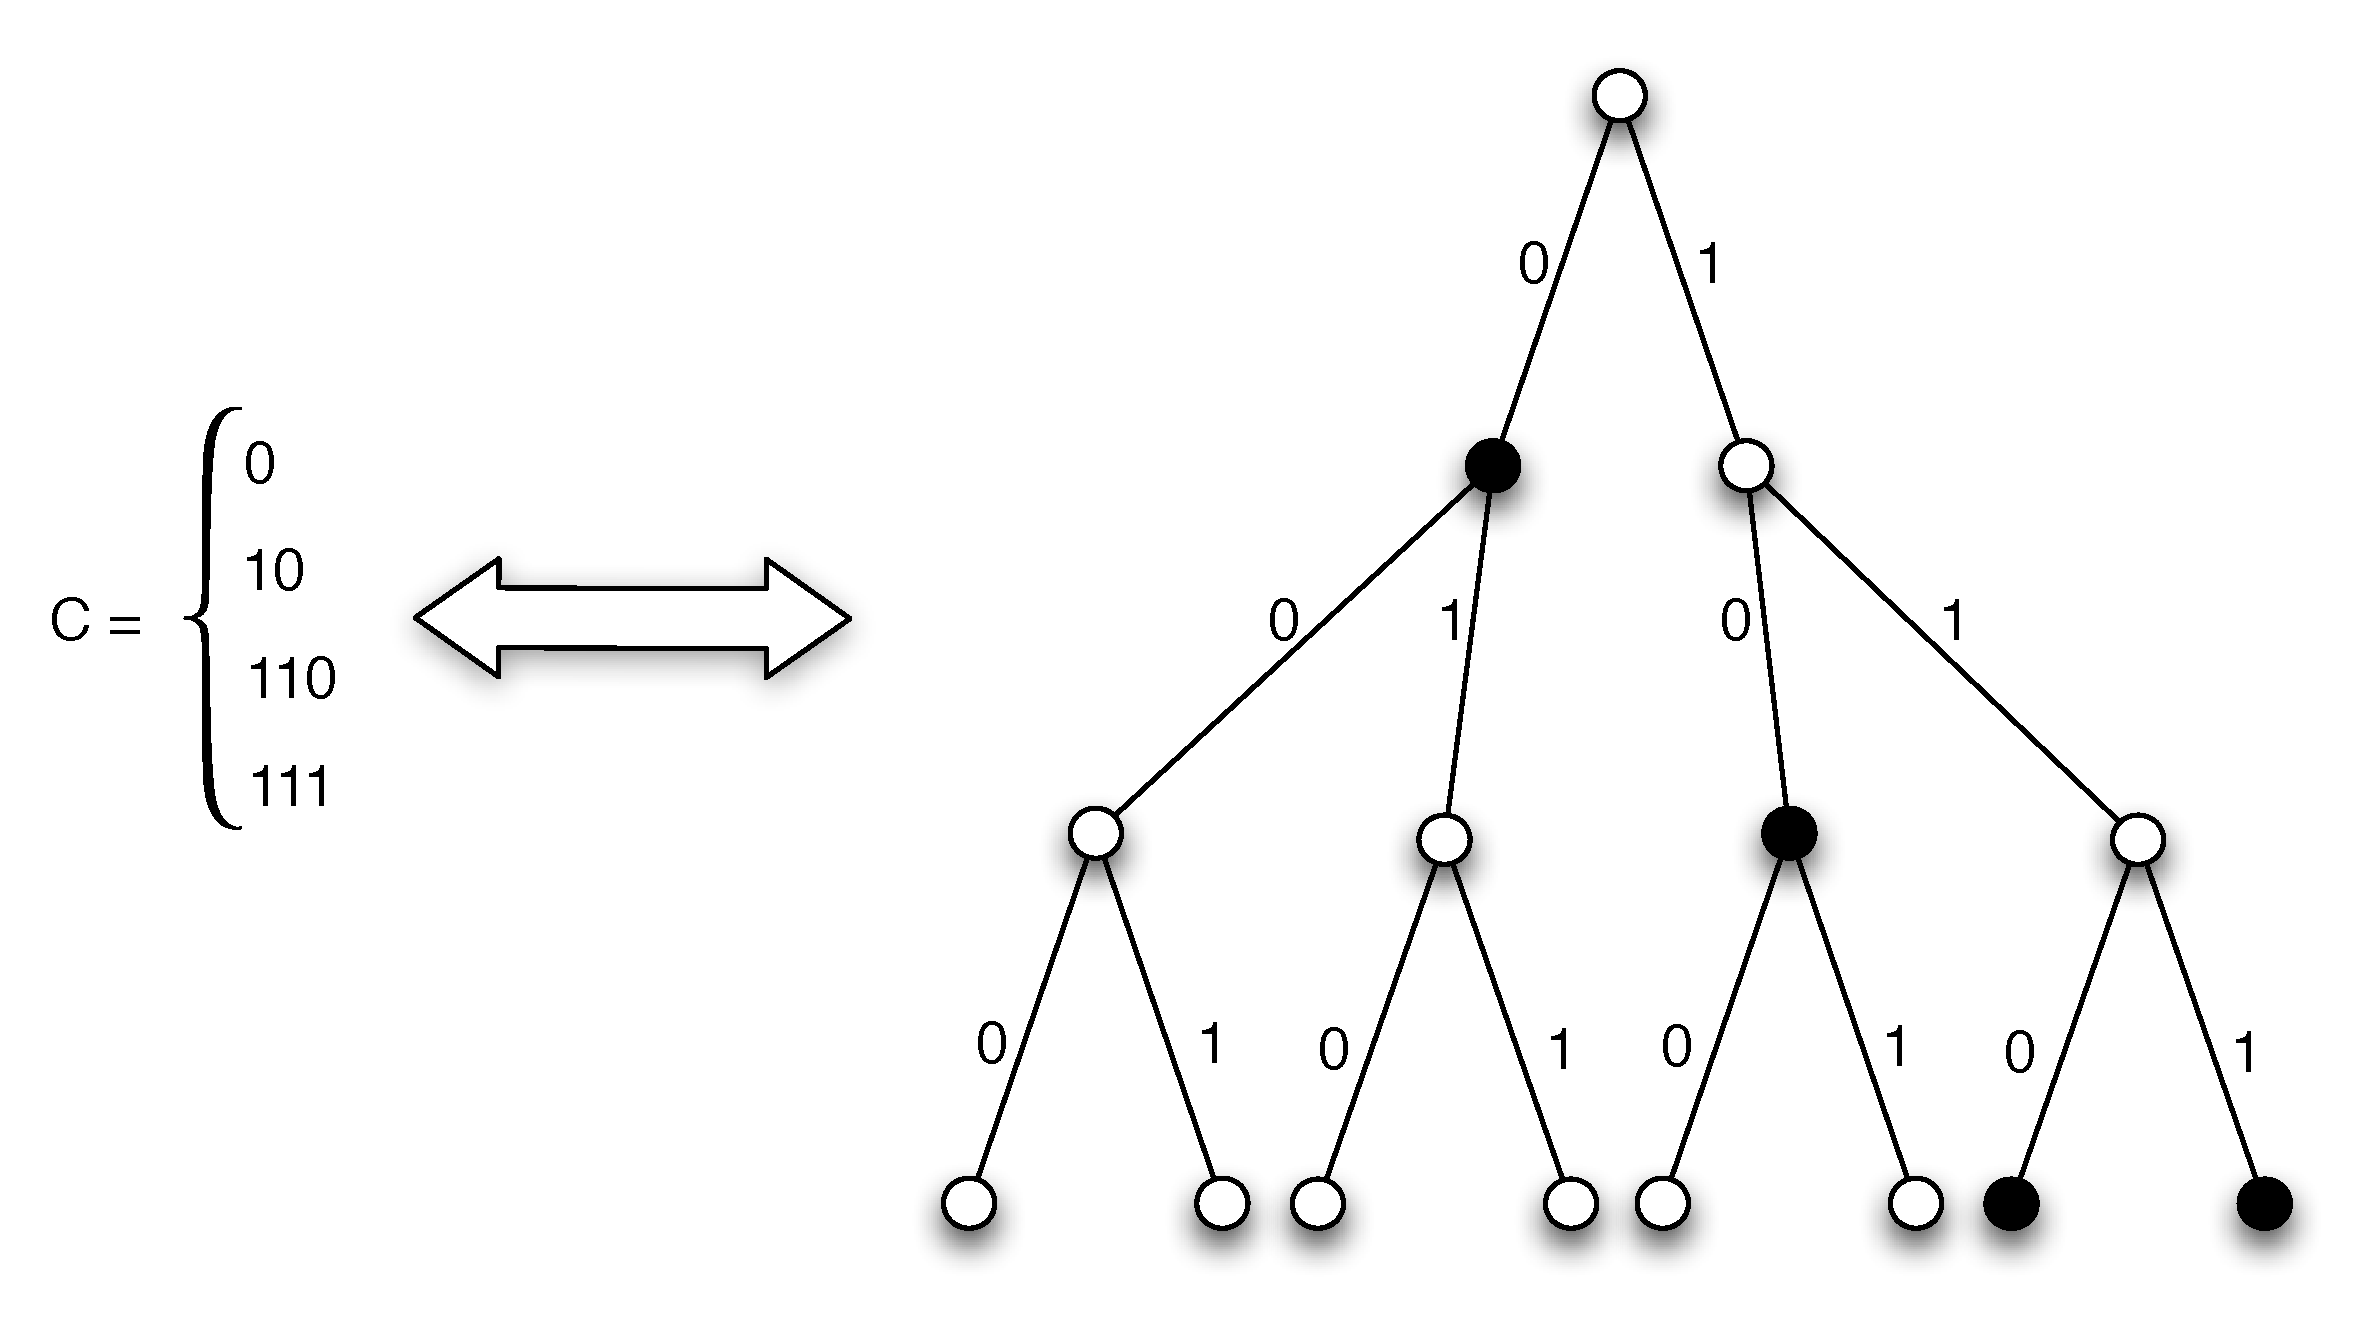
\includegraphics[width=\textwidth]{img/kraft.pdf}
\caption{Esempio di codice e corrispondente albero binario}
\label{fig:albero}
\end{center}
\end{figure}

Dobbiamo ora dimostrare le due implicazioni:
\begin{description}
\item[\(\Longrightarrow\)]: supponiamo che C sia un codice istantaneo D-ario e assumiamo che le lunghezze delle parole di codice siano ordinate in maniera crescente:
\[l_1 \leq l_2 ... \leq l_n\]
Dobbiamo  quindi dimostrare che vale la disuguaglianza del teorema.
Poiché il codice è istantaneo, nessuna parola di codice è prefisso di qualcun'altra. Nella rappresentazione dell'albero, quindi, preso il sottoalbero che fa capo ad una parola di codice, nessun altro vertice corrispondente ad altre parole di codice è contenuto in tale sottoalbero. Di conseguenza i sottoalberi radicati nei vertici delle varie parole di codice non si intersecano.

Siamo ora interessati al numero di foglie di ogni sottoalbero (che fa capo ad una parola di codice). E' facile osservare che un albero 
D-ario ha \(D^{h}\) foglie, con h profondità dell'albero. Ma in questo caso la profondità è pari alla lunghezza della parola di codice più lunga, l'albero avrà dunque \(D^{l_n}\) foglie. Poiché i vari sottoalberi non si intersecano, deve essere:
\[
 \mid I_1 \mid + \mid I_2 \mid + ... + \mid I_n \mid \le D^{l_n}
\]

\begin{figure}[htbp]
\begin{center}
	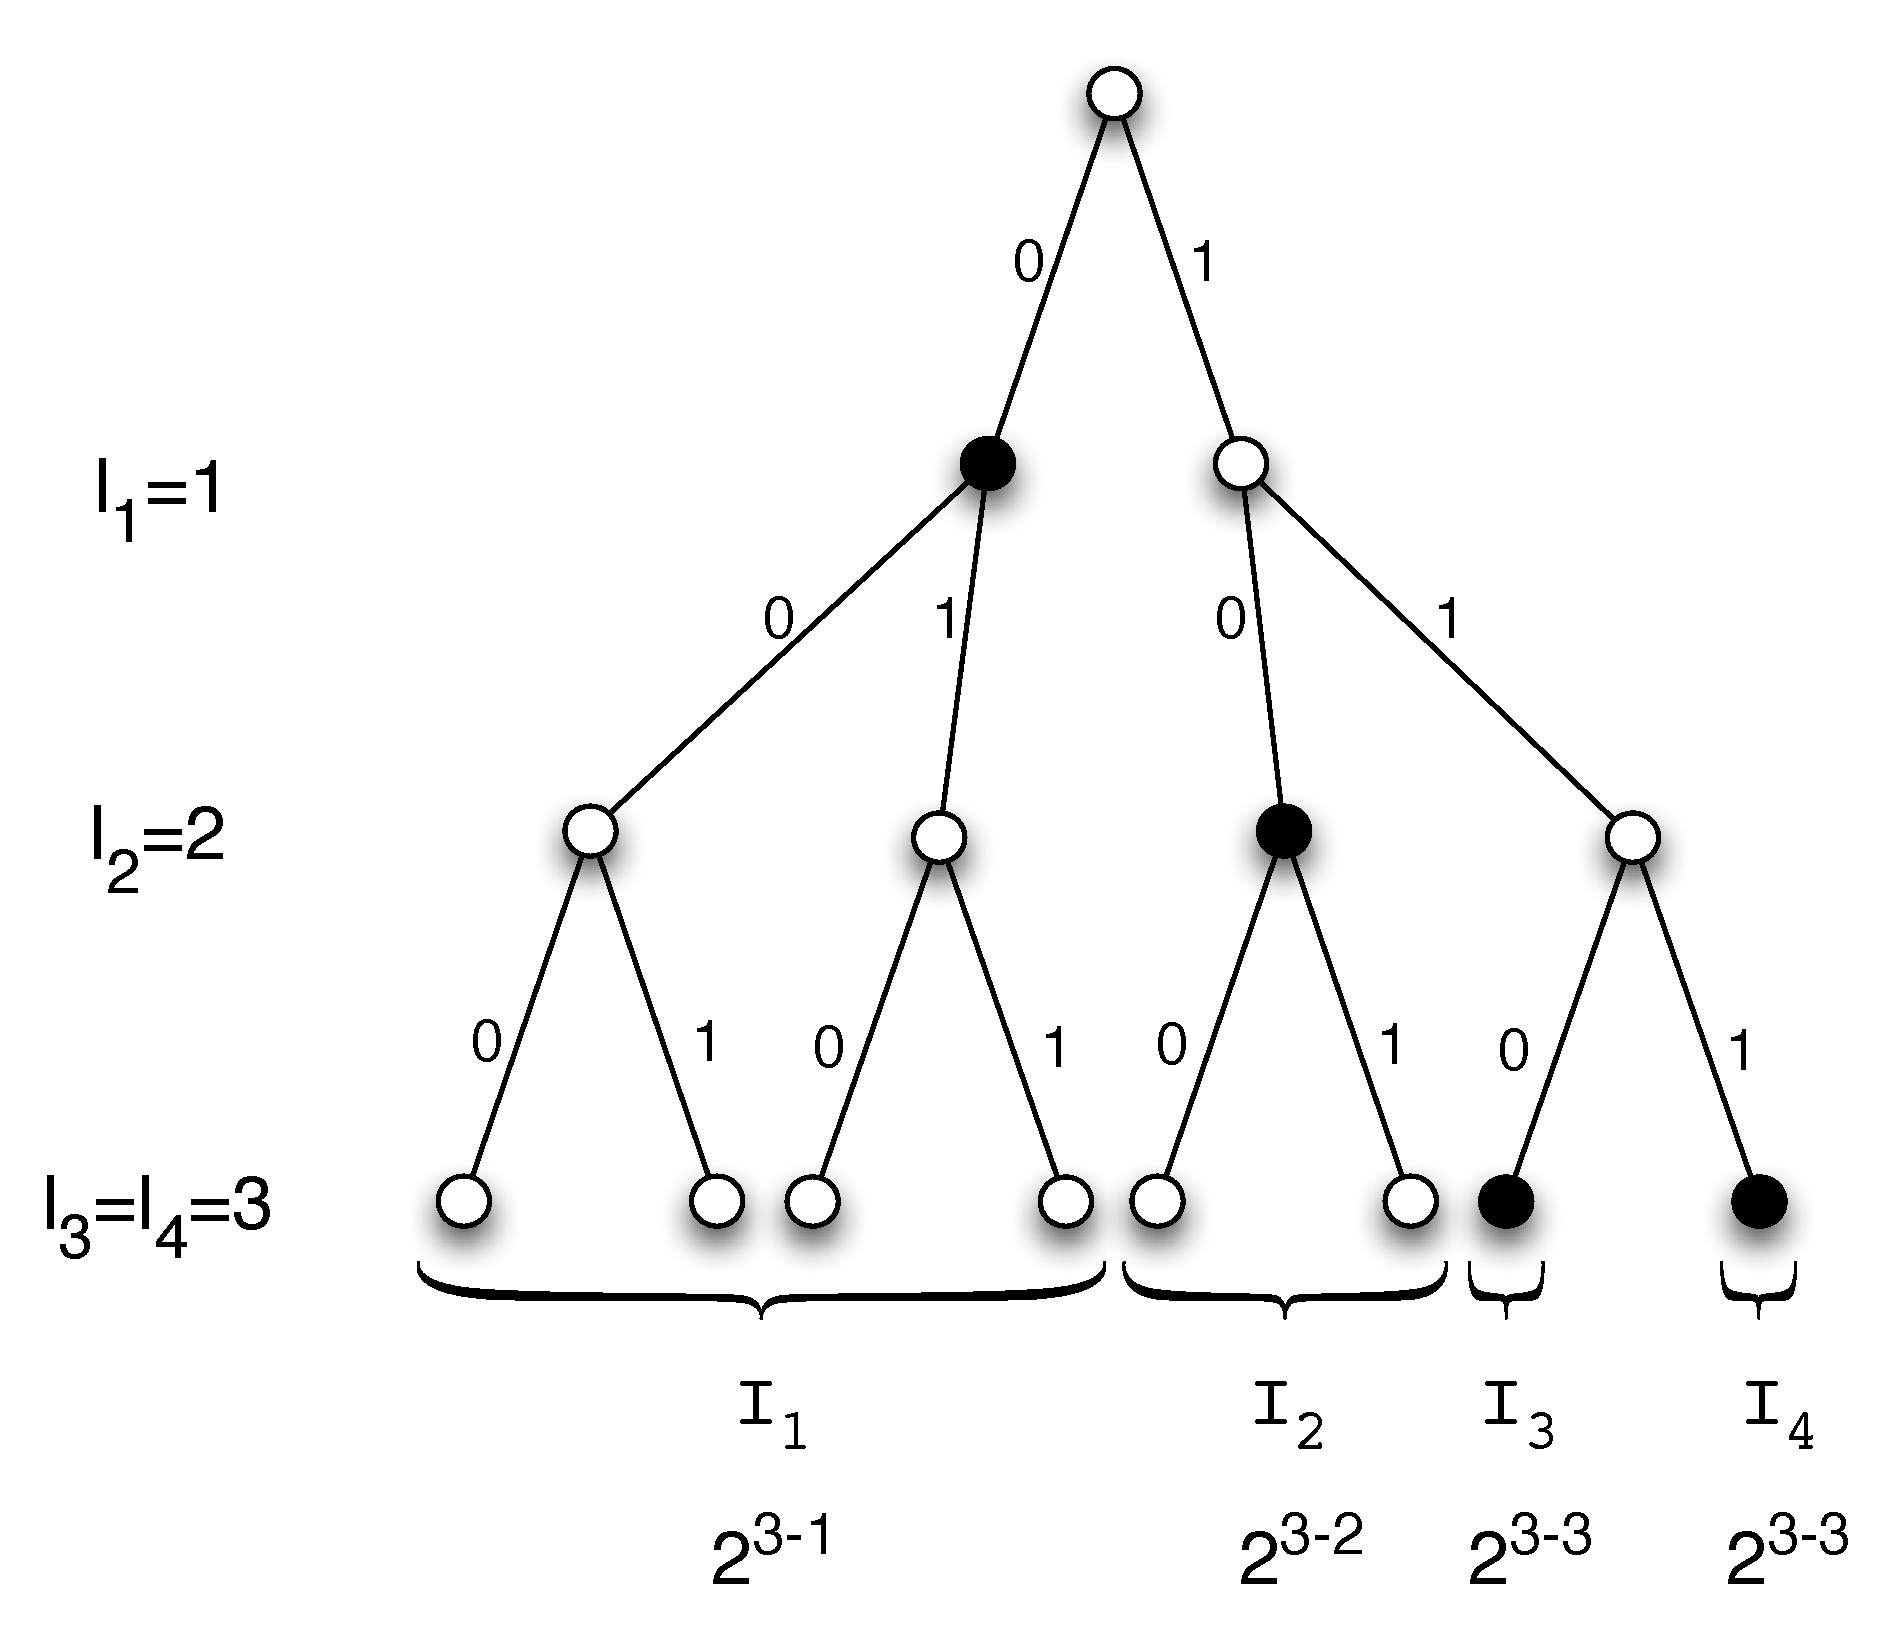
\includegraphics[width=0.7\textwidth]{img/kraft2.pdf}
\caption{Esempio di albero binario associato ad un codice, con varie quantità evidenziate}
\label{fig:albero2}
\end{center}
\end{figure}

Dove con $\mid I_i \mid$ abbiamo indicato il numero di foglie del sottoalbero corrispondente alla parola di codice i.
Per ricavare tale numero, è possibile utilizzare ancora la formula \(D^{h}\). Questa volta però l'altezza è quella del sottoalbero 
che fa capo alla parola i. Per come è costruito l'albero, si ricava che tale altezza vale $l_n-l_i$ (figura \ref{fig:albero2}).

Risulta quindi:
\[ D^{l_n- l_1} + D^{l_n- l_2} + ... D^{l_n- l_n} \leq D^{l_n}\]

Da cui:
\[\begin{split}
 &\sum_{i = 1}^n D^{l_n-l_i} \leq D^{ln} \\
 \Rightarrow &\sum_{i = 1}^n D^{l_n} \cdot D^{-l_i} \leq D^{l_n} \\
 \Rightarrow &D^{l_n} \sum_{i = 1}^n D^{-l_i} \leq D^{l_n} \\
 \Rightarrow &\sum_{i = 1}^n D^{-l_i} \leq 1
 \end{split}
\]

\item[\(\Longleftarrow\)]: supponiamo che valga:
\[\sum_{i = 1}^n D^{-l_i} \leq 1\]
con \(l_1 \leq l_2 ... \leq l_n\) e dimostriamo come sia possibile costruire un codice istantaneo con tali lunghezze.
A tal scopo, costruiamo un codice con il seguente algoritmo:
\begin{enumerate}
\item Presa la prima foglia da sinistra non compresa in un sottoalbero (tra quelli evidenziati nel punto 2), risali fino al livello \(l_i\)
\item Aggiungi la sequenza associata ad \(l_i\) all'insieme delle parole di codice (ed evidenzia il suo sottoalbero)
\item Se non hai raccolto n parole di codice, torna ad 1
\end{enumerate}
Il codice così ottenuto è istantaneo, poichè non ci sono intersezioni fra i sottoalberi corrispondenti alle parole di codice. 
Un esempio dell'applicazione dell'algoritmo è riportato in figura \ref{fig:albero3}.

\begin{figure}[htbp]
\begin{center}
	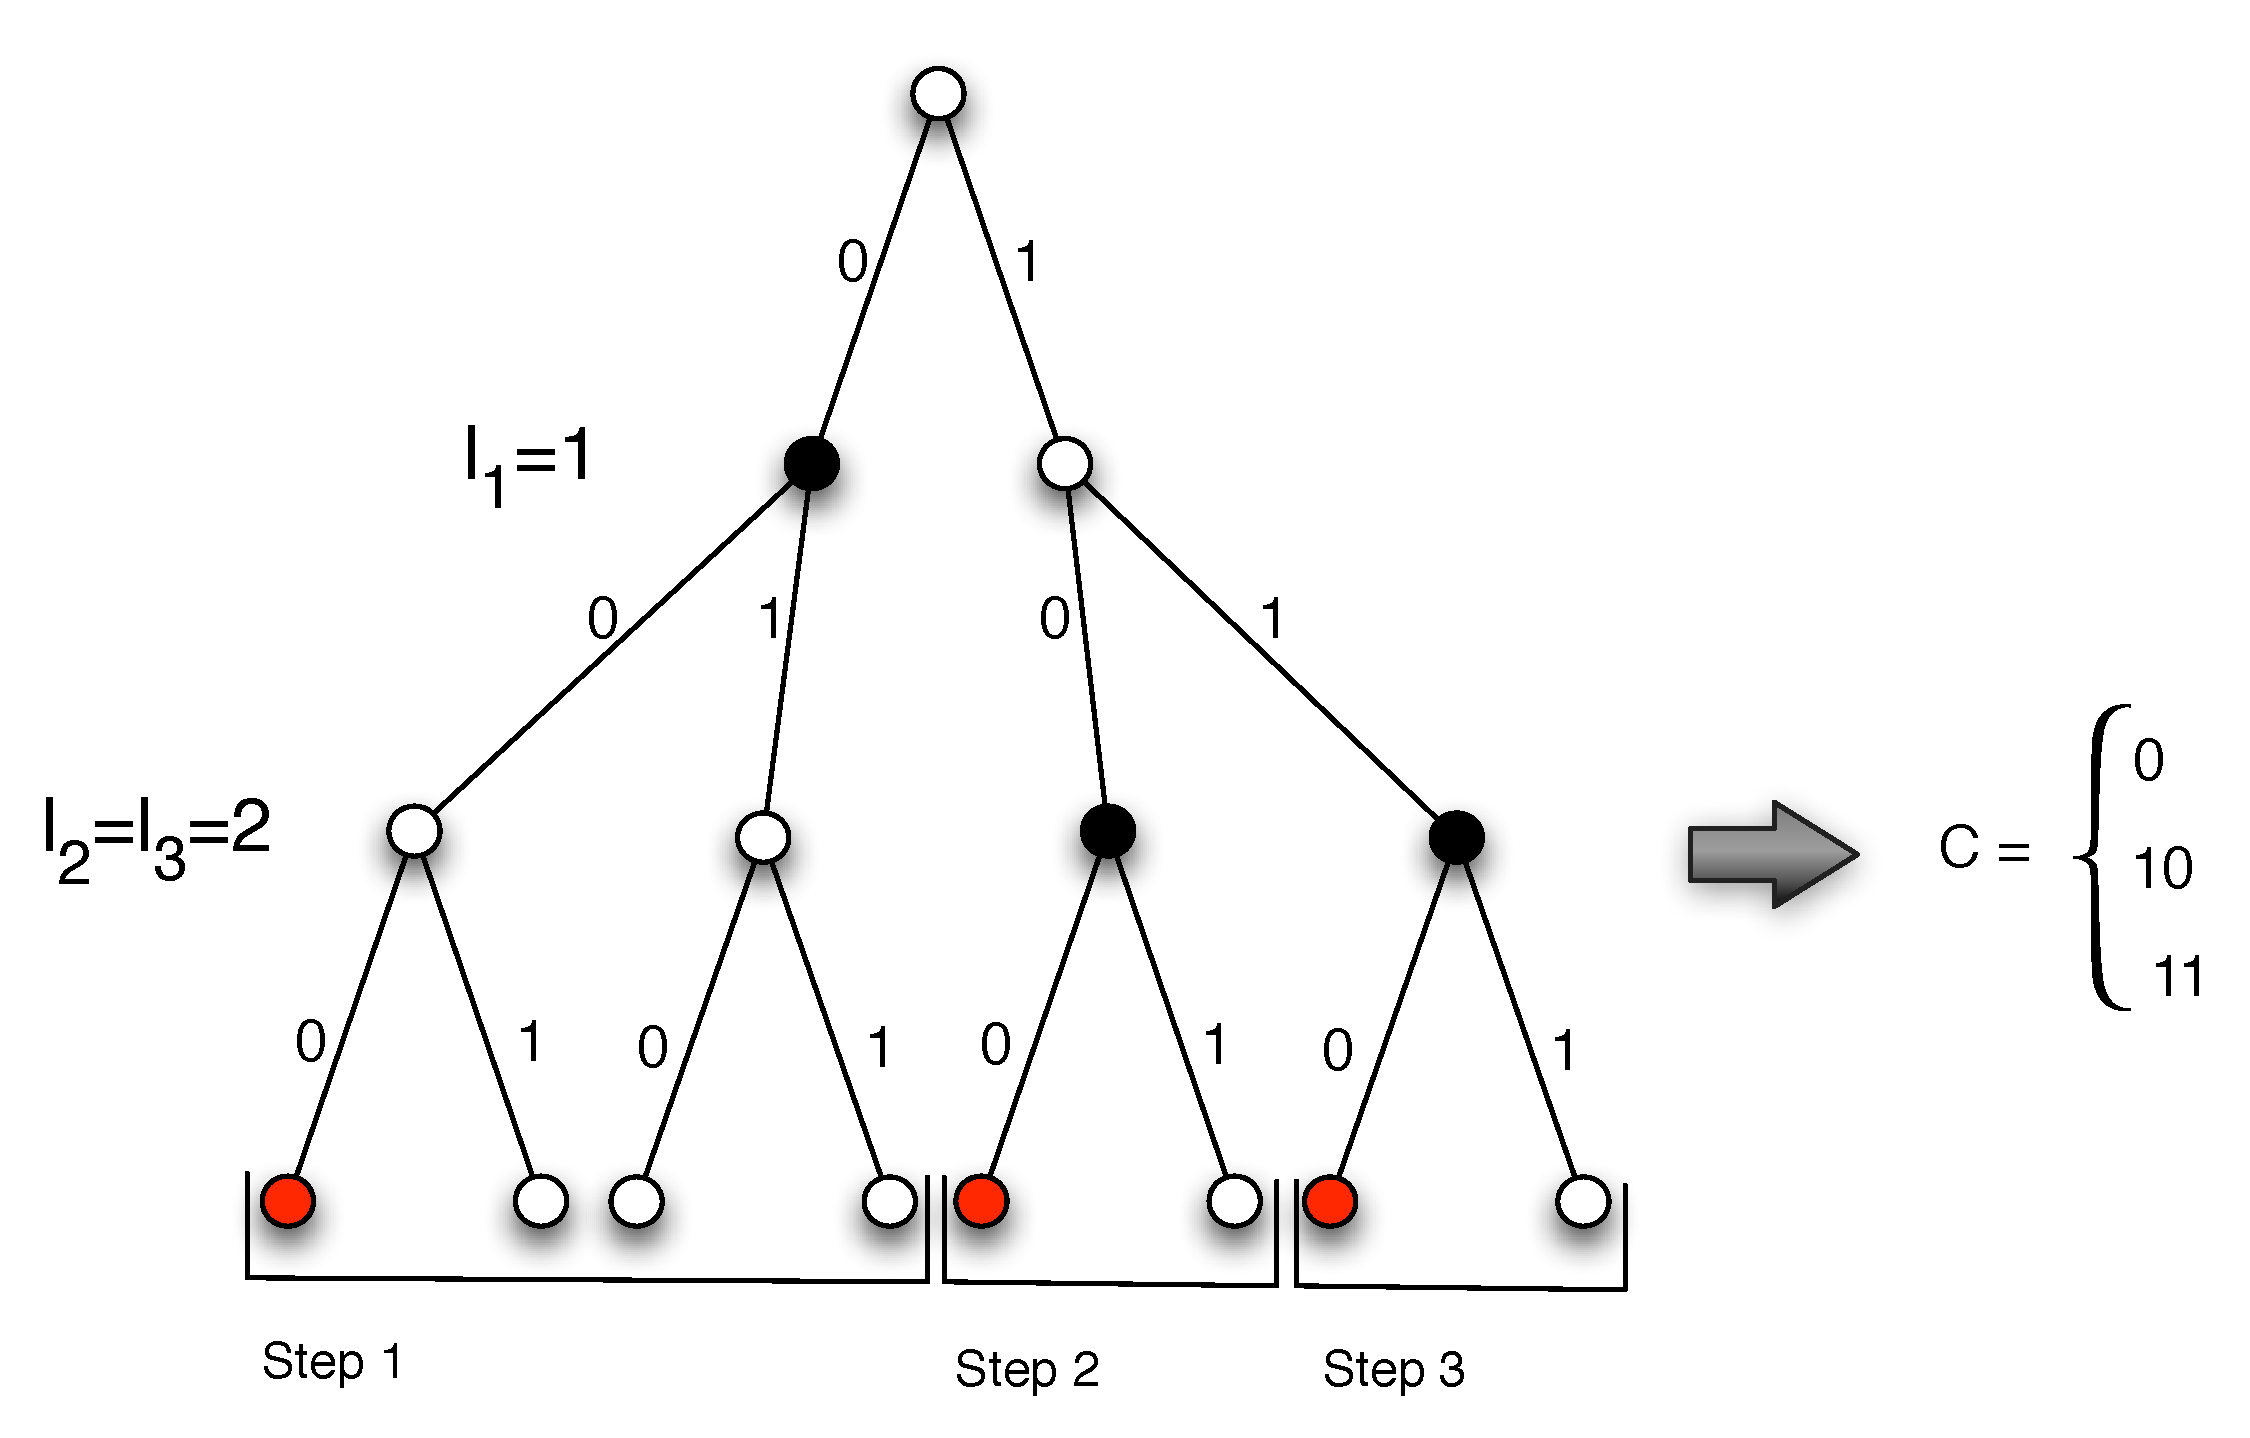
\includegraphics[width=0.9\textwidth]{img/kraft3.pdf}
\caption{Esempio dell'algoritmo per generare il codice istantaneo}
\label{fig:albero3}
\end{center}
\end{figure}

Prima di poter concludere la dimostrazione, è fondamentale risolvere una questione importante. Dobbiamo infatti essere sicuri che ci siano sempre foglie disponibili da cui scegliere ad ogni iterazione dell'algoritmo.
Ovvero l'insieme delle foglie non disponibili (perché facente parti di un sottoalbero) deve essere strettamente 
minore delle foglie totali.
Il numero totale di foglie, come visto prima, è $D^{ln}$. Il numero di foglie non disponibili al passo 0 è 0 (sono tutte disponibili), al passo 1 è $D^{ln-l1}$, al passo 2 è $D^{ln-l1}+D^{ln-l2}$, al passo j è $\sum_{i = 1}^j D^{ln-l_j}$.
Deve quindi essere:
\[
 \forall k=1..n-1 \ : \ \sum_{i = 1}^k D^{ln-l_i} < D^{ln} 
\]

In maniera analoga all'implicazione precedente abbiamo che:
\[
 \begin{split}
  & \sum_{i = 1}^n D^{-l_i} \leq 1 \\
  \Rightarrow & D^{ln} \sum_{i = 1}^n D^{-l_i} \leq D^{ln} \\
  \Rightarrow & \sum_{i = 1}^n D^{ln-l_i} \leq D^{ln}  
 \end{split}
\]

Poiché D è positivo:
\[
\forall i=1..n \ : \ D^{ln-l_i} > 0
\]
Da cui:
\[
  D^{ln-l_1} < D^{ln-l_1} + D^{ln-l_2} < ... < \sum_{i = 1}^{n-1} D^{ln-l_i}  < \sum_{i = 1}^n D^{ln-l_i} \leq D^{ln}  
\]

Quindi esiste sempre una foglia disponibile ad ogni passo dell'algoritmo.
\end{description}
\end{proof}
\end{teorema}

\subsection{Disuguaglianza di McMillan}
Prima di presentare la disuguaglianza, forniamo un lemma utili per la dimostrazione:

\begin{lemma}
 \[
  \forall \alpha > 0 \ : \ \lim_{n \to \infty} \sqrt[n]{\alpha}=1
 \]
\label{lemmaMillan}
\end{lemma}


\begin{teorema}[Disuguaglianza di McMillan]
Condizione necessaria e sufficiente \textbf{affinchè sia possibile} costruire un codice univocamente decodificabile D-ario (ossia un codice costruito su un alfabeto di D simboli) con lunghezza di parola \(l_1, l_2 ... l_n\) è:
\[\sum_{i = 1}^n D^{-l_i} \leq 1\]
\label{macmillan} 

\begin{proof}
Dobbiamo ora dimostrare le due implicazioni:
\begin{description}
\item[\(\Longleftarrow\)]: 
Banale. La disuguaglianza è identica a quella di Kraft. Pertanto possiamo costruire un codice istantaneo, che come abbiamo già visto è anche UD.
\item[\(\Longrightarrow\)]:
Supponiamo di aver costruito un codice $C: \ \X \to D^*$ univocamente decodificabile.
Indicando con l(x) la lunghezza della parola di codice associata ad $x \in X$, dobbiamo dimostrare che:

\[\sum_{x \in \X} D^{-l(x)} \leq 1\]

Consideriamo l'estensione k-esima ($k>1$) di C, $C^k : \X^k \to D^*$.
Poichè C è UD, la sua estensione k-esima sarà non singolare (per definizione di codice UD [\ref{codiceUD}]).
Consideriamo poi la potenza k-esima della parte sinistra della disuguaglianza:
\[\begin{split}
&\left[ \sum_{x \in \X} D^{-l(x)} \right]^k \\
 =& \sum_{a_1 \in \X} D^{-l(a_1)} \sum_{a_2 \in \X} D^{-l(a_2)} ... \sum_{a_k \in \X} D^{-l(a_k)} \\
 =&\sum_{a_1 \in \X} \sum_{a_2 \in \X} ... \sum_{a_k \in \X} \left [ D^{-l(a_1)} D^{-l(a_2)} ... \ D^{-l(a_k)} \right ] \\
 =&\sum_{\bar{a} \in \X^k} D^{-l(\bar{a})}
\end{split}
\]

Dove $\bar{a}=(a_1,a_2,..a_k)$ e $l(\bar{a})=l(a_1)+l(a_2)+...+l(a_k)$

Definiamo ora la sequenza più lunga in X:
\[
 l_{max} = max \{l(x) | x \in \X \}
\]
Definiamo poi l'insieme delle sequenze in $X^k$ di lunghezza m:
\[
 A_m^k=\{ \bar{x} \in X^k \mid l(\bar{x})=m \}
\]
E il numero di tali sequenze:
\[
 {\alpha}_m^k=| A_m^k |
\]
Possiamo allora riscrivere la sommatoria precedente, ordinandola in base alle lunghezze delle parole:
\[
 \sum_{\bar{a} \in \X^k} D^{-l(\bar{a})}=\sum_{m=1}^{k l_{max}} {\alpha}_m^k D^{-m}
\]

Poiché $C^k$ è non singolare deve essere:
\[\alpha_m^k \leq D^m\] 
Infatti $D^m$ è il numero di sequenze lunghe m che possono costruire con D simboli. Affinché $\alpha_m^k$ sia più grande, 
dovrebbero per forza esserci due sequenze uguali (cosa impossibile, perché appunto $C^k$ è non singolare).
Pertanto:
\[\begin{split}
 & \sum_{m=1}^{k l_{max}} {\alpha}_m^k D^{-m} 
 \le \sum_{m=1}^{k l_{max}} D^m D^{-m} \\
 =&\sum_{m=1}^{k l_{max}} 1 
 =k l_{max}
  \end{split}
\]

Riassumendo:
\[
 \forall k>1 \ : \ \left[ \sum_{x \in \X} D^{-l(x)} \right]^k \le k l_{max}
\]

Facendo ora la radice k-esima:
\[
\forall k>1 \ : \ \sum_{x \in \X} D^{-l(x)} \le \sqrt[k]{k} \sqrt[k]{l_{max}}
\]
Poiché la disuguaglianza vale per ogni k, varrà anche per k che tende ad infinito.
Possiamo allora utilizzare il lemma \ref{lemmaMillan} per ottenere:
\[
 \sum_{x \in \X} D^{-l(x)} \le 1
\]

che conclude la dimostrazione.

\end{description}
\end{proof}
\end{teorema}


\section{Codici}
\subsection{Limite alla lunghezza di un codice}
Abbiamo già introdotto il concetto di efficienza di un codice. In particolare, abbiamo evidenziato come un codice efficiente debba 
avere una lunghezza (media) piccola. Tuttavia, questa osservazione ci consente solo di confrontare tra loro due codici, ma non riusciamo 
a determinare se una data lunghezza è ``buona'' o meno.
Il seguente teorema fornisce un limite inferiore alla lunghezza di codice. E' importante notare che anche un codice ottimale può 
(e come si vedrà è quello che accade) non riuscire sempre a raggiungere tale limite.

\begin{teorema} Sia C un codice D-ario univocamente decodificabile, per la variabile aleatoria 
$X \sim p(X_i)=p_i$. Allora:
\begin{itemize}
\item[(i)]
$
 L(C) \ge H_D(X) = \frac{H(X)}{log(D)}
$
\item[(ii)]
$
 L(C) = H_D(X) \iff \forall x_i \in X: -log_D(p(x_i))=l(x_i)
$
\end{itemize}
\label{limitelcodice}
\begin{proof}
\mbox{}

\begin{description}
\item[(i)]: 
Per la definizione di lunghezza di codice [\ref{lunghezza}] e di entropia:
\[
 L(C)=\sum_{i=1}^n p_i l_i \\ H_D(X)=-\sum_{i=1}^n p_i log_D(p_i)
\]

\noindent
Da cui:
\[ \begin{split}
 L(C) - H_D(X) &=\sum_{i=1}^n p_i l_i + \sum_{i=1}^n p_i log_D(p_i) \\
               &=-\sum_{i=1}^n p_i log_D(D^{-l_i}) + \sum_{i=1}^n p_i log_D(p_i) \\
               &=\sum_{i=1}^n p_i log_D \left( \frac{p_i}{D^{-l_i}} \right)  \\
 \end{split}
\]

\noindent
Costruisco ora una distribuzione di probabilià Q:
\[
 \forall i=1..n \ \ q_i=\frac{D^{-l_i}}{C} \\ con \ C=\sum_{k=1}^n D^{-l_k}
\]

\noindent
E da cui (semplice passaggio algebrico):
\[
 D^{-li}=q_i C
\]

\noindent
Q è proprio una una distribuzione di probabilità, poiché:
\begin{enumerate}
 \item $\forall i=1..n \ q_i >0$ Infatti D (la base delle potenze) è sempre positivo.
 \item $\displaystyle\sum_{i=1}^n q_i=1$ Infatti:
  \[
   \sum_{i=1}^n q_i=\sum_{i=1}^n \frac{D^{-l_i}}{C}= \frac{1}{C} \sum_{i=1}^n D^{-l_i} =\frac{1}{C} \ C = 1
  \]

\end{enumerate}

Posso dunque introdurre la distribuzione Q nella formula precedente:
\[ \begin{split}
  & \sum_{i=1}^n p_i log_D \left( \frac{p_i}{D^{-l_i}} \right)  \\
  =&\sum_{i=1}^n p_i log_D \left( \frac{p_i}{C q_i} \right)  \\
  =&\sum_{i=1}^n p_i log_D \left( \frac{p_i}{q_i} \right) + \sum_{i=1}^n p_i log_D \left( \frac{1}{C} \right) \\      
  =&\sum_{i=1}^n p_i log_D \left( \frac{p_i}{q_i} \right) + log_D \left( \frac{1}{C} \right) \sum_{i=1}^n p_i \\
  =&\sum_{i=1}^n p_i log_D \left( \frac{p_i}{q_i} \right) + log_D \left( \frac{1}{C} \right)\\
 \end{split}
\]

Ora accade che la prima parte è una distanza di Kullback-Leibler (def. \ref{distkl}), quindi il termine è maggiore o uguale a 0 (Teorema \ref{leibler}).
C è sicuramente minore di 1. Per ipotesi infatti il codice è UD, quindi vale la disuguaglianza di McMillan (Teorema \ref{macmillan}).
Segue quindi che anche la seconda parte è maggiore o uguale a 0.
Quindi:
\[
 L(C) - H_D(X) \ge 0 \Rightarrow L(C) \ge H_D(X)
\]
\item[(ii)]: 
Utilizzando quanto ricavato nel punto (i), per avere uguaglianza deve essere:
\[
 \sum_{i=1}^n p_i log_D \left( \frac{p_i}{q_i} \right) + log_D \left( \frac{1}{C} \right)=0
\]

Ma poiché entrambi i termini sono maggiori o uguali a 0 ( risultato del punto (i) ), deve essere:
\[
 \sum_{i=1}^n p_i log_D \left( \frac{p_i}{q_i} \right)=0 \\ log_D \left( \frac{1}{C} \right)=0
\]

Da cui:
\[
 log_D \left( \frac{1}{C} \right)=0 \Rightarrow \frac{1}{C}=1 \Rightarrow C=1
\]

Ed inoltre:
\[\begin{split}
  & \sum_{i=1}^n p_i log_D \left( \frac{p_i}{q_i} \right)=0 \\
  \Rightarrow & \forall i=1..n \ log_D \left( \frac{p_i}{q_i} \right)=0 \\
  \Rightarrow & \forall i=1..n \: \ p_i=q_i \\
  \Rightarrow & \forall i=1..n \ : \ p_i=q_i=\frac{D^{-li}}{C} \\
  \Rightarrow & \forall i=1..n \ : \ p_i=\frac{D^{-li}}{C} \\
  \Rightarrow & \forall i=1..n \ : \ p_i=D^{-li} \\
  \end{split}
\]

Riassumendo deve quindi valere che:
\[
 \forall i=1..n \ : \ p_i=D^{-li}
\]

\end{description}
\end{proof}
\end{teorema}

Il teorema appena visto, ci dice in sostanza che sarà possibile raggiungere il limite inferiore per la lunghezza di codice (che è l'entropia), solamente quando la distribuzione di probabilità ha un particolare andamento.
Vista l'importanza di queste considerazioni, a tali distribuzioni di probabilità sarà dato un nome.

\begin{definizione}
 $\bar{p} \in \Delta_n=\{\bar{x} \in R^n \mid x_i \ge 0 \sum_{i=1}^n x_i=1\}$ si dice \textbf{D-adica} se:
\[
 \forall i=1..n \ : \ log_D \left ( \frac{1}{p_i} \right ) \in N
\]
Oppure in maniera equivalente (semplice passaggio algebrico):
\[
 \exists \ l_i \in N \ : \ p_i=D^{-l_i}
\]


\end{definizione}


\subsection{Codice di Shannon}
Come abbiamo visto nel paragrafo precedente, esiste un limite inferiore alla lunghezza di codice.
Il codice di Shannon, cerca di avvicinarsi a questo limite.
Tuttavia non si tratta di un codice ottimale. E' infatti possibile costruire (in alcuni casi) dei codici con 
lunghezza inferiore a quelli del codice di Shannon.

\begin{definizione}[Codice di Shannon]
Data una v.a. $X \sim p(X_i)=p_i$, si dice codice di Shannon ($C_S$) un codice D-ario per cui:
\[
 \forall i \in X: \ l_i=\left \lceil log_D \left (\frac{1}{p_i} \right) \right \rceil
\]

\end{definizione}

\begin{proposizione}E' possibile costruire un codice di Shannon univocamente decodificabile
 \begin{proof}
  Per la definizione del simbolo di intero superiore:
  \[
   \forall x: x \le \lceil x \rceil < x+1
  \]
   Dai cui:
   \[\begin{split}
    & log_D \left( \frac{1}{p_i} \right) \le l_i < log_D \left( \frac{1}{p_i} \right)+1 \\
    \Rightarrow & -l_i \le -log_D \left( \frac{1}{p_i} \right) \\
    \Rightarrow & -l_i \le log_D(p_i) \\
    \Rightarrow & D^{-l_i} \le p_i \\
    \Rightarrow & \sum_{i=1}^n D^{-l_i} \le \sum_{i=1}^n p_i \\
    \Rightarrow & \sum_{i=1}^n D^{-l_i} \le 1
     \end{split}
   \]
   
   \noindent
   A questo punto, per la disuguaglianza di McMillan [\ref{macmillan}], è possibile costruire un codice UD.
 \end{proof}

\end{proposizione}

La proposizione precedente ci dice che possiamo costruire un codice di Shannon UD. Ciò è di fondamentale 
importanza, in quanto (come abbiamo ribadito più volte), un codice non UD è ambiguo (e quindi poco utile).
A questo punto ci interessa sapere quanto il codice di Shannon sia efficiente.
Una prima informazione è fornita dal seguente teorema.

\begin{teorema}
\[
 H_D(X) \le L(C_S) < H_D(X)+1
\]
\begin{proof}
\[\begin{split}
 & l_i=\left \lceil log_D \left (\frac{1}{p_i} \right) \right \rceil \\
 \Rightarrow & log_D \left ( \frac{1}{p_i} \right ) \le l_i < log_D \left ( \frac{1}{p_i} \right ) + 1 \\
 \Rightarrow & p_i log_D \left ( \frac{1}{p_i} \right ) \le p_i l_i < p_i log_D \left ( \frac{1}{p_i} \right ) + p_i \\ 
 \Rightarrow & \sum_{i=1}^n p_i log_D \left ( \frac{1}{p_i} \right ) \le \sum_{i=1}^n  p_i l_i 
                < \sum_{i=1}^n  p_i log_D \left ( \frac{1}{p_i} \right ) + \sum_{i=1}^n p_i \\ 
 \Rightarrow & H_D(X) \le L(C_S) < H_D(X)+1
 \end{split}
\]
\end{proof}
\label{codiceshannon}
\end{teorema}

Il teorema dice in sostanza che il codice è ``buono'', in quanto si avvicina molto al limite inferiore (l'entropia in base D).
Tuttavia il codice non è ottimale, come è facile dimostrare tramite un controesempio.

\begin{proposizione}
 Il codice di Shannon non è ottimale
\begin{proof}
 Consideriamo il seguente controesempio: Sia $\X=\{1,2,3\}$ e D=2 (codice binario). Sia inoltre 
 $p(x_1)=2/3$, $p(x_2)=2/9$, $p(x_3)=1/9$.
 Allora:
\[\begin{split}
 L(C_S) &= \sum_{i=1}^3 p_i l_i \\
        &= \frac{2}{3} \left \lceil log \left (\frac{3}{2} \right) \right \rceil + 
           \frac{2}{9} \left \lceil  log \left (\frac{9}{2} \right) \right  \rceil +
           \frac{1}{9} \biggl \lceil log \left (9            \right) \biggr \rceil \\
        &= \frac{2}{3} + \frac{2}{3} + \frac{4}{3} \\
        & \simeq 1.78 
  \end{split}
\]
 
 Costruiamo ora un codice C' migliore di $C_S$, provando quindi che $C_S$ non è ottimale.
 Poniamo C'(1)=0, C'(2)=10, C'(3)=11. Quindi $l_1=1$, $l_2=2$, $l_3=2$. Il codice è banalmente UD.
 Calcoliamo la sua lunghezza:

\[\begin{split}
 L(C') &= \sum_{i=1}^3 p_i l_i \\
        &= 1 \frac{2}{3} + 
           2 \frac{2}{9} +
           2 \frac{1}{9} \\
        &= \frac{4}{3}\\
        & \simeq 1.33
  \end{split}
\]

Chiaramente $L(C') < L(C_S)$, quindi $C_S$ non è ottimale

\end{proof}
\end{proposizione}

Per quanto riguarda il controesempio formulato nella dimostrazione della proposizione, è interessante calcolare anche l'entropia di X:

\[\begin{split}
 H(X) &= H \left( \frac{2}{3},\frac{2}{9},\frac{1}{9} \right) \\
      &=\frac{2}{3}log \left (\frac{3}{2} \right) + \frac{2}{9}log \left (\frac{9}{2} \right) 
+ \frac{1}{9}log \left (9 \right) \\
 & \simeq 1.22
  \end{split}
\]

L'entropia è minore di C' (abbiamo infatti dimostrato che è un limite inferiore). Si noti tuttavia che C' nell'esempio precedente 
è ottimale, tuttavia non si riesce a raggiunge il valore dell'entropia (X non è infatti 2-adica). Si noti infine che, quando 
X è D-adica, il codice di Shannon è ottimale. Succede infatti che il logaritmo è un numero naturale e quindi la lunghezza coincide 
con l'entropia.

\subsection{Codice di Huffman}
Vediamo ora un altro codice, che questa volta è ottimale. Si tratta del codice di Huffman.
A differenza del codice di Shannon, in questo caso viene fornito un algoritmo, che consente di costruire il codice.
L'idea di fondo è che ai simboli meno probabili debbano essere assegnate le parole di codice più lunghe (e di egual lunghezza).
Per semplicità utilizziamo un esempio per descrivere il funzionamento dell'algoritmo.
Consideriamo il procedimento in tabella \ref{tab:huffman1}:
\begin{itemize}
 \item L'insieme dei simboli è $s_1$,$s_2$,$s_3$,$s_4$,$s_5$ con probabilità rispettivamente 
       0.4, 0.3, 0.1, 0.1, 0.06, 0.04
 \item Si ordinano le probabilità in maniera decrescente e si ottiene $S_0$
 \item Si ``accorpano'' i due simboli meno probabili (che sono gli ultimi due in virtù dell'ordinamento).
       Si costruisce quindi $S_1$, sommando le probabilità di questi due simboli. In figura, la probabilità 
       che si ottengono come somma sono quelle cerchiate.
 \item Si ripete il procedimento fino a che non rimangono solamente due probabilità (in questo caso al passo $S_4$)
 \item Si assegna 0 al primo simbolo ed 1 al secondo, costruendo $C_4$
 \item Per costruire $C_3$, si riporta il codice per le probabilità non cerchiate (in questo caso 1 per la probabilità 0.4).
       Per la probabilità cerchiata invece si riporta il codice ad entrambi i simboli che si erano accorpati.
       Si aggiunge poi 0 per il primo simbolo ed 1 per il secondo.
 \item Si ripete il procedimento fino ad ottenere $C_0$
 \item $C_0$ è il codice cercato
\end{itemize}

\begin{table}[htbp]
  \begin{center}
   \begin{tabular}{l|| l|l|| l|l|| l|l|| l|l|| l|l}
	 & $S_0$ & $C_0$  & $S_1$ & $C_1$  & $S_2$ & $C_2$  & $S_3$ & $C_3$  & $S_4$ & $C_4$\\
       \hline
	$s_1$ & 0.4 & 1     & 0.4 & 1     & 0.4 & 1   & 0.4 & 1 & $ \boxed{0.6}$ & 0  \\ 
	$s_2$ & 0.3 & 00    & 0.3 & 00    & 0.3 & 00  & 0.3 & 00 & 0.4 & 1 \\ 
	$s_3$ & 0.1 & 011   & 0.1 & 011   & $\boxed{0.2}$ & 010 & $\boxed{0.3}$ & 01 & &\\ 
        $s_4$ & 0.1 & 0100  & 0.1 & 0100  & 0.1 & 011 & & & & \\ 
        $s_5$ & 0.06 & 01010 & $\boxed{0.1}$ & 0101 & & & & &\\ 
        $s_6$ & 0.04 & 01011 & & & & & & &\\ 
    \end{tabular}
     
     \caption{Esempio del funzionamento dell'algoritmo di Huffman}
    \label{tab:huffman1}
  \end{center}
\end{table}

Si noti che l'algoritmo consente di scegliere liberamente quale debba essere la somma delle due probabilità.
E' quindi possibile, a seconda delle scelte fatte, ottenere codici diversi.
Nell'esempio in tabella \ref{tab:huffman1}, avremo potuto infatti decidere che la somma di 0.2 e 0.1 in $S_3$, era il primo
0.3 e non il secondo. Per chiarire questo punto, si osservi l'esempio in tabella \ref{tab:huffman2}. Sebbene la variabile X 
(simboli con loro probabilità) sia la stessa, il codice ottenuto è completamente diverso.

\begin{table}[htbp]
  \begin{center}
   \begin{tabular}{l|| l|l|| l|l|| l|l|| l|l|| l|l}
	 & $S_0$ & $C_0$  & $S_1$ & $C_1$  & $S_2$ & $C_2$  & $S_3$ & $C_3$  & $S_4$ & $C_4$\\
       \hline
	$s_1$ & 0.4 & 1     & 0.4 & 1     & 0.4 & 1   & 0.4 & 1 & $ \boxed{0.6}$ & 0  \\ 
	$s_2$ & 0.3 & 01    & 0.3 & 01    & 0.3 & 01  & $\boxed{0.3}$ & 00 &           0.4 & 1 \\ 
	$s_3$ & 0.1 & 0000   & $\boxed{0.1}$ & 001   & $\boxed{0.2}$ & 000 & 0.3 & 01 & &\\ 
        $s_4$ & 0.1 & 0001  & 0.1 & 0000  & 0.1 & 001 & & & & \\ 
        $s_5$ & 0.06 & 0010 & 0.1 & 0001 & & & & &\\ 
        $s_6$ & 0.04 & 0011 & & & & & & &\\ 
    \end{tabular}
     
     \caption{Esempio del funzionamento dell'algoritmo di Huffman}
    \label{tab:huffman2}
  \end{center}
\end{table}

Persino la lunghezza delle varie parole di codice non è esattamente la stessa. Nel secondo caso infatti 4 parole di codice sono lunghe 4, mentre nel primo caso solamente una lo è. Tuttavia, entrambi i codici sono ottimali.

E' interessante notare che a volte non è necessario terminare tutto il procedimento. Se infatti accade che per alcune distribuzioni di probabilità (ottenute durante il procedimento) si conosce un codice ottimale, lo si può inserire. Si riduce così il numero di passi da 
eseguire. Naturalmente è difficile avere a disposizione un codice ottimale ``direttamente''. Tuttavia se la distribuzioni di probabilità è D-adica, come abbiamo visto, possiamo utilizzare il codice di Shannon.
Consideriamo l'esempio in tabella \ref{tab:huffman3}. In questo caso $S_1$ è D-adica.
E' facile dunque calcolare le lunghezze delle parole di codice, che sono banalmente 1,2,3,3. Infatti 
log(2)=1,log(4)=2,log(8)=3. Basta quindi costruire un codice UD che rispetti queste lunghezze e proseguire da questo punto in poi con l'algoritmo di Huffman.

\begin{table}[htbp]
  \begin{center}
   \begin{tabular}{l|| l|l|| l|l}
	 & $S_0$ & $C_0$  & $S_1$ & $C_1$\\
       \hline
	$s_1$ & 0.5 & 0     & 0.5 & 0 \\ 
	$s_2$ & 0.25 & 10    & 0.25 & 10 \\ 
	$s_3$ & 0.125 & 110   & 0.125 & 110\\ 
        $s_4$ & 0.100 & 1110  & $\boxed{0.125}$ & 111 \\ 
        $s_5$ & 0.025 & 1111 &  &   \\ 
    \end{tabular}
     
     \caption{Esempio del funzionamento dell'algoritmo di Huffman, semplificato dal fatto che $S_1$ è D-adica}
    \label{tab:huffman3}
  \end{center}
\end{table}


Dimostriamo ora che il codice di Huffman è ottimale. Prima però introduciamo alcuni lemmi che saranno utili durante la dimostrazione.
\begin{proposizione}[Regola di Morse]
\mbox{}

 Sia:
 \[
  C: \X \to \D^*
 \]
  un codice ottimale. Allora:
\[
 \forall x,y \in \X: p(x)>p(y) \Rightarrow l(x) \le l(y)
\]
\begin{proof}
\mbox{}

 Supponiamo per assurdo che:
\[
 \exists x,y \in \X: p(x)>p(y) \Rightarrow l(x) > l(y)
\]

 \noindent
 Costruiamo allora un codice C' la cui lunghezza è inferiore a quella di C, dimostrando quindi che C 
 non è ottimale. Sia:

 \[
  C': \X \to \D^*
 \]

 un codice definito nel modo seguente:
 \[
  \forall z \in \X \
  C'(z)=
   \begin{cases} 
     C(z) & \mbox{se } z \ne x \land z \ne y  \\ 
     C(x) & \mbox{se } z=y \\
     C(y) & \mbox{se } z=x
   \end{cases} 
 \]

\noindent
Ovvero C' è identico a C, salvo per il fatto che le due parole di codice per i simboli x e y sono state scambiate.
Si ha che:

\[ \begin{split}
 L(C)-L(C') &=\sum_{z \in \X} p(z) l(z) - \sum_{z \in \X} p(z) l'(z) \\
            &=\sum_{z \in \X} p(z)[l(z)-l'(z)] \\
            &=\sum_{z \in \X}^{
                    z \ne x \land z\ne y} p(z)[l(z)-l(z)] + p(x)[l(x)-l'(x)] + p(y)[l(y)-l'(y)] \\
            &=p(x)[l(x)-l'(x)] + p(y)[l(y)-l'(y)] \\
            &=p(x)[l(x)-l(y)] + p(y)[l(y)-l(x)] \\
            &=p(x)[l(x)-l(y)] - p(y)[l(x)-l(y)] \\
            &=[p(x)-p(y)][l(x)-l(y)]
   \end{split}
\]

\noindent
Ma p(x) e p(y) sono positive in quanto probabilità e per ipotesi $p(x) > p(y)$. Avevamo inoltre supposto che $l(x) > l(y)$. Pertanto:
\[
 [p(x)-p(y)][l(x)-l(y)] > 0 \Rightarrow L(C)-L(C')>0 \Rightarrow L(C')<L(C)
\]

\noindent
Quindi la lunghezza di C' è inferiore a C, pertanto C non può essere ottimale. Assurdo.

\end{proof}

\end{proposizione}

La regola di Morse ci dice in sostanza che, per avere un codice ottimale, è necessario che a simboli più probabili siano assegnate 
parole di codice più corte. Nel famoso codice Morse infatti alla lettera E (che in un testo in lingua inglese è la più frequente) è assegnato un solo simbolo. 

\begin{proposizione}
 Sia C un codice istantaneo ed ottimale. Allora le 2 parole di codice più lunghe hanno la stessa lunghezza.
\begin{proof}
 Supponiamo per assurdo che ciò non sia vero. Sia allora b la parola più lunga ed a la seconda parola più lunga, quindi $l(a)<l(b)$.
 Posso allora costruire un codice C' identico a C, salvo per il fatto che b è troncata ai primi l(a) simboli.
 Il codice è banalmente istantaneo (infatti a non era un prefisso di b). Tuttavia la sua lunghezza è inferiore a quella di C, 
 poiché $l(a)<l(b)$. Pertanto C non è ottimale. Assurdo.
\end{proof}

\end{proposizione}

\begin{osservazione}
 E' sempre possibile costruire un codice ottimale, in cui le 2 parole più lunghe differiscono solo per l'ultimo bit.
\label{diff1bit}
\end{osservazione}


\begin{teorema}[Teorema di Huffman]
L'algoritmo di Huffman restituisce un codice:
\begin{itemize}
\item[(i)] Istantaneo
\item[(ii)] Ottimale
\end{itemize}
\begin{proof}
\mbox{}

\begin{itemize}
\item[(i)]
Per induzione.
Il caso base è il primo codice costruito dall'algoritmo ($C_n$). Per il funzionamento dell'algoritmo il codice è formato unicamente da due simboli, pertanto è banalmente istantaneo.
Per il passo induttivo, dimostriamo che se $C_k$ è istantaneo, allora lo è anche $C_{k-1}$.
Ciò è banalmente vero, in quanto $C_{k-1}$ è uguale a $C_k$ (che è istantaneo per ipotesi), tranno per il fatto che una parola di codice è stata ``sdoppiata'' in due. Tuttavia queste due parole non sono prefisso di altre (per come sono costruite), pertanto anche $C_k$ è istantaneo.
\item[(ii)]
Per induzione. Il caso base è il primo codice costruito dall'algoritmo ($C_n$). Poiché le 2 parole di codice sono formate unicamente da un simbolo, il codice è banalmente ottimale. Per il passo induttivo, dimostriamo che se $C_{k+1}$ è ottimale, allora lo è anche $C_{k}$.
In tabella \ref{tab:huffdim} è rappresentato un passo dell'algoritmo di Huffman.

\begin{table}[htbp]
  \begin{center}
   \begin{tabular}{l || l|l|| l|l || l}
	 ... & $S_k$ & $C_k$  & $S_{k+1}$ & $C_{k+1}$ & ...\\
       \hline
	...& $s_0$          $p_0$          & $w_0$ & $s_0$ $p_0$      & $w_0$ & ... \\ 
	...& $s_1$          $p_1$          & $w_1$ & $s_1$ $p_1$      & $w_1$ & ... \\ 
	...& $s_2$          $p_2$          & $w_2$ & $s_2$ $p_2$      & $w_2$ & ...\\
        ...& $...$          ...            & ...   & ...   ...      & ... & ...\\  
        ...& $s_{\alpha 0}$ $p_{\alpha 0}$ & $w_{\alpha 0}$ & $s_{\alpha}$ $p_{\alpha}$ & $w_{\alpha}$ & \\ 
        ...& $s_{\alpha 1}$ $p_{\alpha 1}$ & $w_{\alpha 1}$ &             &  &   \\ 
    \end{tabular}
     
     \caption{Situazione in un passo dell'algoritmo di Huffman}
    \label{tab:huffdim}
  \end{center}
\end{table}

Per come funziona l'algoritmo di Huffman, si ha che:
\[ \begin{split}
 &p_{\alpha} =p_{\alpha0}+p_{\alpha1} \\
 &w_{\alpha0} =w_{\alpha}0 \\
 &w_{\alpha1}=w_{\alpha}1 \\
 &l(w_{\alpha0})=l(w_{\alpha1})=l(w_{\alpha})+1
 \end{split}
\]

Possiamo ora calcolare la lunghezza dei vari codici intermedi costruiti dall'algoritmo.
Indichiamo con $L_k$ la lunghezza del codice k-esimo, ovvero $L_k=L(C_k)$.
Allora:

\[\begin{split}
 L_{k+1}&=p_0 l(w_0) + p_1 l(w_1) + ... + p_{\alpha} l(w_{\alpha})
  \end{split}
\]

\[ \begin{split}
 L_{k} &=p_0 l(w_0) + p_1 l(w_1) + ... + p_{\alpha0} l(w_{\alpha0}) + p_{\alpha1} l(w_{\alpha1}) \\
       &=p_0 l(w_0) + p_1 l(w_1) + ... + p_{\alpha0} [l(w_{\alpha})+1] + p_{\alpha1} [l(w_{\alpha})+1] \\
       &=p_0 l(w_0) + p_1 l(w_1) + ... + [p_{\alpha0}+p_{\alpha1}][l(w_{\alpha})+1] \\
       &=p_0 l(w_0) + p_1 l(w_1) + ... + p_{\alpha}[l(w_{\alpha})+1] \\
 \end{split}
\]

\[\begin{split}
 L_{k+1}-L_{k}&=p_0 l(w_0) + p_1 l(w_1) + ... + p_{\alpha} l(w_{\alpha}) \\
              &-p_0 l(w_0) - p_1 l(w_1) - ... - p_{\alpha}[l(w_{\alpha})+1] \\
              &=p_{\alpha} l(w_{\alpha}) - p_{\alpha}[l(w_{\alpha})+1] \\
              &=-p_{\alpha}
 \end{split}
\]

\[
 L_{k+1}=L_{k}-p_{\alpha}
\]



\noindent
Supponiamo ora per assurdo che $C_{k}$ non sia ottimale. Ciò equivale a dire che esiste un codice 
$\bar{C}_k$, la cui lunghezza è inferiore a quella di $C_k$:
\[
 \exists \ \bar{C}_k : \bar{L}_k < L_k
\]

Per l'osservazione \ref{diff1bit}, è sempre possibile costruire un codice ottimale per cui le due parole più 
lunghe differiscono solo nell'ultimo bit. Consideriamo pertanto che $\bar{C}_k$ sia un codice per cui vale questa proprietà.
Se ora applichiamo l'algoritmo di Huffman ``al contrario'', a partire da $\bar{C}_k$, possiamo costruire un codice 
$\bar{C}_{k+1}$. Tale codice sarà uguale a $\bar{C}_k$, ma con le due parole più lunghe fuse in un unico simbolo 
(private dell'ultimo bit).
Esattamente come nel caso precedente, si avrà che:
\[
 \bar{L}_{k+1}=\bar{L}_{k}-p_{\alpha}
\]
Da cui:
\[\begin{split}
 \bar{L}_{k+1} - L_{k+1}&=\bar{L}_{k}-p_{\alpha} - [L_k-p_{\alpha}] \\
  &=\bar{L}_{k}-p_{\alpha} - L_k+p_{\alpha} \\
  &=\bar{L}_{k}-L_k
 \end{split}
\]

Ma poiché $\bar{L}_k < L_k$, si ha che:
\[
 \bar{L}_k-L_k<0 \Rightarrow \bar{L}_{k+1}-L_{k+1}<0 \Rightarrow \bar{L}_{k+1}<L_{k+1}
\]

Ovvero risulterebbe che $C_{k+1}$ non è ottimale, in quanto $\bar{C}_{k+1}$ ha una lunghezza inferiore.
Ma questo è assurdo, poiché per ipotesi $C_{k+1}$ era ottimale.
Segue quindi che $C_{k}$ è ottimale, concludendo la dimostrazione.

\end{itemize}
\end{proof}
\end{teorema}

Abbiamo utilizzato il codice di Huffman solamente con alfabeti binari, tuttavia l'algoritmo 
funziona anche nel caso più generale di alfabeti D-ari. Anche la dimostrazione di ottimalità può essere estesa 
per considerare questo caso (non sarà fatto).

Naturalmente l'algoritmo necessita di qualche modifica, nel caso di alfabeti con D simboli. In maniera abbastanza intuitiva, invece di prendere gli ultimi 2 simboli, si prenderanno gli ultimi D.
Tuttavia c'è un problema evidente: il numero di simboli di partenza, potrebbe non ridursi esattamente a D nell'ultima fase ``forward''.
Per risolvere questo problema, possiamo aggiungere dei simboli fittizzi (con probabilità 0) nella fase iniziale.
Naturalmente bisogna determinare quanti simboli è necessario aggiungere.

L'algoritmo, ad ogni passo della prima fase, accorpa gli ultimi D simboli. Ciò vuol dire che nel passo i ci sono D-1 simboli in meno rispetto al passo i-1. Infatti ne vengono eliminati D, ma se ne aggiunge uno (che è appunto l'accorpamento dei D simboli).
Facendo uno schema riassuntivo:
\[\begin{split}
 S_0 \ &: \ n \ simboli  \\
 S_1 \ &: \ n-(D-1) \ simboli \\
 S_2 \ &: \ n-(D-1)-(D-1)=n-2(D-1) \ simboli \\
 S_3 \ &: \ n-3(D-1) \ simboli \\
 S_i \ &: \ n-i(D-1) \ simboli
   \end{split}
\]

Poiché nell'ultima fase vogliamo avere D simboli, deve essere che:
\[
 \exists \ k \ge 1 : D=n-k(D-1)
\]

Da cui:
\[
 n=D+k(D-1)=(D-1)+k(D-1)+1=(K+1)(D-1)+1
\]

Ovvero n deve essere congruo ad 1 (in modulo D-1):

\[
 n \equiv 1 \  mod(D-1)
\]

\noindent
In sostanza devo aggiungere una serie di simboli, finché tale condizione non è soddisfatta.

\bigskip
\noindent
\textbf{Esempio}
Consideriamo D=\{0,1,2,3\} ed una sorgente con 11 simboli.
Dobbiamo quindi trovare $n \ge 11$ tale che:
\[
 n \equiv 1 \  mod(3)
\]
Il risultato è chiaramente 13 (infatti 3*4+1=13), dobbiamo quindi aggiungere 2 simboli fittizzi.
L'algoritmo di Huffman in un caso con questi parametri è riportato in tabella \ref{tab:huffmanD}.

\begin{table}[htbp]
  \begin{center}
   \begin{tabular}{l|l|| l|l|| l|l|| l|l}
	 $S_0$ & $C_0$  & $S_1$ & $C_1$  & $S_2$ & $C_2$  & $S_3$ & $C_3$ \\
       \hline
	0.22 & 2   & 0.22 & 2       & $\boxed{0.23}$& 1 & $\boxed{0.40}$ & 0  \\ 
	0.15 & 3   & 0.15 & 3       & 0.22          & 2  & 0.23 & 1 \\ 
	0.12 & 00  & 0.12 & 00      & 0.15          & 3  & 0.22 & 2 \\ 
        0.10 & 01  & 0.10 & 01      & 0.12          & 00 & 0.15 & 3 \\ 
        0.10 & 02  & 0.10 & 02      & 0.10          & 01 & &\\ 
        0.08 & 03  & 0.08 & 03      & 0.10          & 02 & &\\
        0.06 & 11  & $\boxed{0.07}$ & 10 & 0.08     & 03 & &\\  
        0.05 & 12  & 0.06 & 11 & & &\\
        0.05 & 13  & 0.05 & 12 & & &\\
        0.04 & 100 & 0.05 & 13 & & &\\    
        0.03 & 101 & & & & &\\    
        \hline
        0 & 102 & & & & &\\    
        0 & 103 & & & & &\\    
    \end{tabular}
     
     \caption{Esempio del funzionamento dell'algoritmo di Huffman con 4 simboli}
    \label{tab:huffmanD}
  \end{center}
\end{table}

\section{1° Teorema di Shannon}
Come abbiamo visto, il codice di Huffman fornisce un algoritmo per costruire un codice ottimale.
In sostanza quindi, sembrerebbe che il limite di efficienza sia stato raggiunto e meglio di così non si possa fare per comprimere 
l'informazione. E' stato anche visto che se la distribuzione X non è D-adica, nemmeno un codice ottimale (e.g. Huffman) riesce a raggiungere (relativamente alla lunghezza) il valore dell'entropia (che è un limite inferiore).

Analizzando più attentamente la questione, ci si accorge che fortunatamente si può fare di meglio. Fino ad ora infatti abbiamo 
considerato i simboli emessi dalla sorgente singolarmente. E' interessante invece vedere cosa si riesce ad ottenere se si considerano 
insiemi di simboli. Si vuole in sostanza fare una cosiddetta ``Codifica a pacchetto''.

Per inquadrare meglio questa idea, facciamo un esempio. Supponiamo che la sorgente generi due simboli A e B, con probabilità rispettivamente 2/3 ed 1/3. Il miglior codice possibile è banalmente quello che utilizza un unico bit per simbolo (tabella 
\ref{tab:codpac1}).

\begin{table}[htbp]
  \begin{center}
   \begin{tabular}{c|c l}
	 $\X$ & p  & $C^1$ \\
       \hline
	A & 2/3 & 0  \\ 
	B & 1/3 & 1 \\ 
    \end{tabular}
     \caption{Un codice per S}
    \label{tab:codpac1}
  \end{center}
\end{table}

Consideriamo ora l'estensione seconda della sorgente, che corrisponde all'emissione di due simboli.
Un codice ottimale è riportato in tabella \ref{tab:codpac2}.

\begin{table}[htbp]
  \begin{center}
   \begin{tabular}{c|c l}
	 $\X^2$ & p  & $C^2$ \\
       \hline
	AA & 4/9 & 0  \\ 
	AB & 2/9 & 10 \\
        BA & 2/9 & 110 \\  
        BB & 1/9 & 111 \\ 
    \end{tabular}
     \caption{Un codice per $S^2$}
    \label{tab:codpac2}
  \end{center}
\end{table}

In maniera analoga possiamo costruire l'estensione terza della sorgente e così via.
Calcoliamo ora la lunghezza dei codici ottimali $C^1$, $C^2$, $C^3$ (quest'ultimo non è stato indicato,ma visto che interessa solo la sua lunghezza può essere costruito con l'algoritmo di Huffman) e l'entropia della variabile X.
Si noti che per lunghezza del codice $C^k$, intendiamo la lunghezza relativamente alla sorgente iniziale. Ovvero, una volta 
calcolata la lunghezza con la formula usuale, è necessario dividere per k. Infatti il codice invia k simboli, ma noi vogliamo considerare la lunghezza per inviare un solo simbolo.
Facendo i dovuti calcoli si ottiene:
\[\begin{split}
 L(C^1)&=1 \\
 L(C^2)& \simeq 0.944 \\
 L(C^3)& \simeq 0.938 \\
 H(X)& \simeq 0.918
 \end{split}
\]

Dai dati che si ottengono, sembrerebbe che l'idea della ``codifica a pacchetto'' sia buona. La lunghezza si riduce, avvicinandosi 
al valore dell'entropia. Cerchiamo ora di formalizzare questa intuizione.

Consideriamo una sorgente senza memoria S $[ \ \{X_i\}_i iid \ ]$ e la sua estensione n-esima $S^n$. Consideriamo poi un codice ottimale per $S^n$. Indichiamo tale codice con $C^n$ e la sua lunghezza con $L^*$.

\noindent
Abbiamo dimostrato (teorema \ref{codiceshannon}) che per il codice di Shannon vale:
\[
 H_D(X) \le L(C_S) < H_D(X)+1
\]

\noindent
Tuttavia, visto che stiamo considerando un codice ottimale, a maggior ragione varrà questa disuguaglianza.
In dettaglio avremo che:
\[
 H_D(X_1..X_n) \le L^* < H_D(X_1..X_n)+1
\]
Da cui:
\[\begin{split} 
 & H_D(X_1..X_n) \le L^* < H_D(X_1..X_n)+1 \\
 \Rightarrow & n H_D(\X) \le L^* < nH_D(\X) + 1 \\
 \Rightarrow & H_D(\X) \le \frac{L^*}{n} < H_D(\X) + \frac{1}{n} \\
 \Rightarrow & \lim_{n \to \infty} \frac{L^*}{n}=H_D(\X)  
  \end{split}
\]

In sostanza quindi, la nostra intuizione era corretta: al crescere del numero di simboli considerati, la lunghezza si avvicina sempre di 
più all'entropia. L'ipotesi che ci ha consentito di ottenere questo risultato è stata quella di indipendenza della variabile X.
E' infatti grazie ad essa che è possibile trasformare $H_D(X_1..X_n)$ in $n H_D(\X)$. Il risultato vale dunque solamente nel caso 
di una sorgente senza memoria.

Proviamo ora a generalizzare i risultati ottenuti, considerando S come processo stazionario S $[ \ \{X_i\}_i \ stazionario \ ]$.
In questo caso si ottiene:
\[
 \begin{split} 
 & H_D(X_1..X_n) \le L^* < H_D(X_1..X_n)+1 \\
 \Rightarrow & \frac{H_D(X_1..X_n)}{n} \le \frac{L^*}{n} < \frac{H_D(X_1..X_n)}{n} + \frac{1}{n} \\
 \Rightarrow & \lim_{n \to \infty} \frac{L^*}{n}=\frac{H_D(X_1..X_n)}{n}=H_D(\bar{X})  
  \end{split}
\]

Il risultato è analogo al precedente, tuttavia questa volta la lunghezza tende al tasso entropico $H_D(\bar{X})$ invece che all'entropia.
Questo risultato è noto come 1° teorema di Shannon (o della codifica di sorgente).

\begin{teorema}[1° teorema di Shannon (o della codifica di sorgente)]
 Sia S una sorgente stazionaria e $S^n$ la sua estensione n-esima, con n qualsiasi. Sia $C^n$ un codice ottimale UD D-ario per $S^n$.
 Allora:
 \[
  \lim_{n \to \infty} \frac{L^*}{n}=H_D(\bar{S})  
 \]

\end{teorema}

\section{Un codice tramite il teorema AEP}
L'AEP è un risultato di grande importanza anche per la costruzione di codici.
In particolare costruiremo un codice binario utilizzando quanto visto nel paragrafo dell'AEP (sez. \ref{aep}).
Il codice sarà formato da due pacchetti (o parti in questo caso), le sequenze tipiche e le sequenze atipiche.
Per distinguere questi due pacchetti, utilizzermo un bit (e.g. 0 sequenza tipica, 1 atipica).
Determiniamo ora il numero di bit necessari per ciascun pacchetto:
\begin{itemize}
 \item Sequenze tipiche: E' stato visto che per il numero di sequenze tipiche vale che:
       \[
        | A_{\epsilon}^n| \le 2^{n(H(X)+\epsilon)}
       \]
       Se identifico quindi ciascuna sequenza con un numero avrò bisogno di al più $2^{n(H(X)+\epsilon)}$ ``numeri''.
       Quindi, poiché siamo nel caso binario, serviranno:
       \[
        log_2 2^{n(H(X)+\epsilon)}=n(H(X)+\epsilon) bit
       \]
       Tuttavia, visto che si potrebbe ottenere un numero reale, è necessario aggiungere un ulteriore bit.
       I bit necessari per codificare le sequenze sono dunque:
       \[
        n(H(X)+\epsilon)+1
       \]


 \item Sequenze atipiche: In questo caso, in maniera abbastanza banale, possiamo considerare un numero di bit sufficiente 
       a codificare tutte le possibili sequenze (che sono $|X^n|$).
       Servono pertanto:
       \[
         log|X^n|=nlog(|X|) \ bit
       \]
       Come nel caso precedente, è necessario un bit aggiuntivo. I bit necessari sono dunque:
       \[
        n log(|X|)+1
       \]

\end{itemize}

Vediamo ora come la lunghezza del codice così costruito sia arbitrariamente vicina all'entropia.


\begin{teorema}
\[
 E \left [ \frac{1}{n} l(X^n) \right] \le H(x)+\delta \ \forall \delta >0 \ ed \ n \ sufficientemente \ grande
\]
\begin{proof}
E' necessario dimostrare che:
\[
 \forall \delta >0, \exists n_o \in N: \ \forall n \ge n_0 \ E \left [ \frac{1}{n} l(X^n) \right] \le H(x)+\delta
\]
 Pongo allora:
\[
 \epsilon=\frac{\delta}{2+log(|X|)} > 0
\]
Inoltre:
 \begin{itemize}
  \item[a)]
   \[
    \lim_{n \to \infty} \frac{2}{n}=0 \Rightarrow \forall \epsilon >0 \ \exists n_1 \in N: \ \forall n>n_1 \ \frac{2}{n} \le \epsilon
   \]
  \item[b)]
   \[
    \lim_{n \to \infty} Pr\{A_{\epsilon}^n\}=1 \Rightarrow \forall \epsilon >0 \ \exists n_2 \in N: \ \forall n>n_2 \ 
Pr\{A_{\epsilon}^n\} \ge 1-\epsilon
   \]
 \end{itemize}

\noindent
Pongo allora $n_0=max(n_1,n_2)$ e considero $n>n_0$.
Vale che:
\[\begin{split}
 E \left [ l(X^n) \right]&=\sum_{x \in X^n} p(\bar{x})l(\bar{x}) \\
 &=\sum_{x \in A_{\epsilon}^n} p(\bar{x})l(\bar{x})  + \sum_{x \in \bar{A}_{\epsilon}^n} p(\bar{x})l(\bar{x}) \\
 &= [n(H(X)+\epsilon)+2]\sum_{x \in A_{\epsilon}^n} p(\bar{x}) + [nlog(|X|)+2]\sum_{x \in \bar{A}_{\epsilon}^n} p(\bar{x}) \\
 &= [n(H(X)+\epsilon)+2] Pr\{A_{\epsilon}^n\} + [nlog(|X|)+2] Pr\{\bar{A}_{\epsilon}^n\} \\
 &= [n(H(X)+\epsilon)+2] Pr\{A_{\epsilon}^n\} + [nlog(|X|)+2] (1-Pr\{A_{\epsilon}^n\}) \\
 &=n(H(X)+\epsilon)Pr\{A_{\epsilon}^n\} + nlog(|X|)(1-Pr\{A_{\epsilon}^n\}) + 2\\
 \end{split}
\]
Ora per il fatto che come tutte le probabilità $0 \le Pr\{A_{\epsilon}^n\} \le 1$ e che vale (b), si ha:
\[\begin{split}
  &n(H(X)+\epsilon)Pr\{A_{\epsilon}^n\} + nlog(|X|)(1-Pr\{A_{\epsilon}^n\}) + 2\\
  \le &n(H(X)+\epsilon) + nlog(|X|)(1-Pr\{A_{\epsilon}^n\}) + 2\\
  \le& n(H(X)+\epsilon) +n log(|X|)\epsilon + 2 \\
   =&n[H(X)+\epsilon+\epsilon log(|X|) + \frac{2}{n}]
  \end{split}
\]
Ora si può utilizzare (a):
\[\begin{split}
   &n[H(X)+\epsilon+\epsilon log(|X|) +\frac{2}{n}]  \\
  \le & n[H(X)+\epsilon+\epsilon log(|X|) +\epsilon]  \\
  =& n[H(X)+\epsilon log(|X|) +2\epsilon]  \\
  =& n[H(X)+\epsilon ( 2+ log(|X|))]  \\
  \end{split}
\]
Sostituiamo ora $\epsilon$:
\[\begin{split}
 & n[H(X)+\epsilon ( 2+log(|X|) )]  \\
 =&n[H(X)+ \frac{\delta}{2+log(|X|)} ( 2+log(|X|) )] \\
 =&n[H(X)+ \delta]
 \end{split}
\]
Riassumendo si ha dunque che:
\[
 E \left [ l(X^n) \right] \le n[H(X)+ \delta]
\]
Dividendo infine per n:
\[
 \frac{1}{n} E \left [ l(X^n) \right] \le H(X)+ \delta \iff E \left [ \frac{1}{n} l(X^n) \right] \le H(X)+ \delta
\]


\end{proof}
\end{teorema}

